\documentclass[preprint,12pt]{elsarticle}

% =======================================================
% PACKAGES
% =======================================================
\usepackage[utf8]{inputenc}
\usepackage[T1]{fontenc}
\usepackage{lmodern}
\usepackage{amsmath,amssymb,amsfonts}
\usepackage{algorithmic}
\usepackage{algorithm}
\usepackage{graphicx}
\usepackage{textcomp}
\usepackage{xcolor}
\usepackage{booktabs}
\usepackage{multirow}
\usepackage{array}
\usepackage{url}
\usepackage{listings}
\usepackage[hidelinks]{hyperref}
\usepackage{microtype}
\usepackage{tikz}
\usepackage{pgfplots}
\pgfplotsset{compat=1.18}
\usetikzlibrary{shapes, arrows.meta, positioning, shadows, calc, chains}

% - Colors -
\definecolor{pipelineBlue}{RGB}{0, 85, 180}
\definecolor{pipelineMagenta}{RGB}{200, 0, 120}
\definecolor{codeGreen}{rgb}{0,0.5,0}
\definecolor{codeGray}{rgb}{0.4,0.4,0.4}
\definecolor{codePurple}{rgb}{0.58,0,0.82}
\definecolor{codeBack}{rgb}{0.97,0.97,0.99}

% - Macros -
\newcommand{\SystemName}{\textsc{Hybrid-Flow}}
\newcommand{\Code}[1]{\texttt{#1}}

% - Listing style -
\lstdefinestyle{customc}{
    language=C,
    backgroundcolor=\color{codeBack},
    basicstyle=\ttfamily\small,
    keywordstyle=\color{pipelineBlue}\bfseries,
    stringstyle=\color{codePurple},
    commentstyle=\color{codeGreen}\itshape,
    numberstyle=\tiny\color{codeGray},
    numbers=left,
    frame=lines,
    breaklines=true,
    tabsize=2,
    captionpos=b
}

% Every number quoted in the text is a macro generated from the raw results
% (hybridflow/results) by hybridflow/hf/report.py, ext_analysis.py and paper_extra.py.
% ---- begin generated/numbers ----
% generated by hf/report.py from results/metrics.json - do not edit by hand
\newcommand{\ablPFourFP}{0}
\newcommand{\ablPFourFone}{91.4\%}
\newcommand{\ablPFourParse}{0.0\%}
\newcommand{\ablPFourPrec}{100.0\%}
\newcommand{\ablPFourRec}{84.1\%}
\newcommand{\ablPFourTok}{332}
\newcommand{\ablPOneFP}{1}
\newcommand{\ablPOneFone}{70.3\%}
\newcommand{\ablPOneParse}{12.5\%}
\newcommand{\ablPOnePrec}{97.8\%}
\newcommand{\ablPOneRec}{54.9\%}
\newcommand{\ablPOneTok}{490}
\newcommand{\ablPThreeFP}{0}
\newcommand{\ablPThreeFone}{91.4\%}
\newcommand{\ablPThreeParse}{0.0\%}
\newcommand{\ablPThreePrec}{100.0\%}
\newcommand{\ablPThreeRec}{84.1\%}
\newcommand{\ablPThreeTok}{368}
\newcommand{\ablPTwoFP}{0}
\newcommand{\ablPTwoFone}{90.7\%}
\newcommand{\ablPTwoParse}{0.0\%}
\newcommand{\ablPTwoPrec}{100.0\%}
\newcommand{\ablPTwoRec}{82.9\%}
\newcommand{\ablPTwoTok}{293}
\newcommand{\agreeQwen}{98.3\%}
\newcommand{\cacheAccCEighty}{79.1\%}
\newcommand{\cacheAccCEightyFive}{77.9\%}
\newcommand{\cacheAccCExact}{80.8\%}
\newcommand{\cacheAccCNinety}{80.2\%}
\newcommand{\cacheAccCNinetyFive}{80.2\%}
\newcommand{\cacheAccFEighty}{80.8\%}
\newcommand{\cacheAccFEightyFive}{80.8\%}
\newcommand{\cacheAccFExact}{80.8\%}
\newcommand{\cacheAccFNinety}{80.8\%}
\newcommand{\cacheAccFNinetyFive}{80.8\%}
\newcommand{\cacheChgEighty}{15}
\newcommand{\cacheChgEightyFive}{9}
\newcommand{\cacheChgExact}{0}
\newcommand{\cacheChgNinety}{1}
\newcommand{\cacheChgNinetyFive}{1}
\newcommand{\cacheFPCEighty}{7}
\newcommand{\cacheFPCEightyFive}{4}
\newcommand{\cacheFPCExact}{0}
\newcommand{\cacheFPCNinety}{0}
\newcommand{\cacheFPCNinetyFive}{0}
\newcommand{\cacheFPFEighty}{0}
\newcommand{\cacheFPFEightyFive}{0}
\newcommand{\cacheFPFExact}{0}
\newcommand{\cacheFPFNinety}{0}
\newcommand{\cacheFPFNinetyFive}{0}
\newcommand{\cacheHitEighty}{34.3\%}
\newcommand{\cacheHitEightyFive}{20.3\%}
\newcommand{\cacheHitExact}{2.3\%}
\newcommand{\cacheHitNinety}{9.9\%}
\newcommand{\cacheHitNinetyFive}{6.4\%}
\newcommand{\cacheHitsEighty}{59}
\newcommand{\cacheHitsEightyFive}{35}
\newcommand{\cacheHitsExact}{4}
\newcommand{\cacheHitsNinety}{17}
\newcommand{\cacheHitsNinetyFive}{11}
\newcommand{\cacheQEighty}{172}
\newcommand{\cacheQEightyFive}{172}
\newcommand{\cacheQExact}{172}
\newcommand{\cacheQNinety}{172}
\newcommand{\cacheQNinetyFive}{172}
\newcommand{\covEvAIOneTwenty}{95.5\%}
\newcommand{\covEvAITwenty}{85.8\%}
\newcommand{\covEvGcc}{19.2\%}
\newcommand{\covEvHBOneTwenty}{91.1\%}
\newcommand{\covEvHBTwenty}{89.0\%}
\newcommand{\covEvHCOneTwenty}{49.3\%}
\newcommand{\covEvHCTwenty}{93.7\%}
\newcommand{\covEvHFiftyOneTwenty}{95.3\%}
\newcommand{\covEvHFiftyTwenty}{93.7\%}
\newcommand{\covEvHOneTwenty}{49.3\%}
\newcommand{\covEvHTwenty}{93.7\%}
\newcommand{\covEvPolly}{8.5\%}
\newcommand{\covEvStatic}{44.1\%}
\newcommand{\covFullGcc}{23.4\%}
\newcommand{\covFullPolly}{6.8\%}
\newcommand{\covFullStatic}{58.6\%}
\newcommand{\evAIOneTwentyFN}{23}
\newcommand{\evAIOneTwentyFP}{38}
\newcommand{\evAIOneTwentyFone}{87.8\%}
\newcommand{\evAIOneTwentyFoneHi}{90.6\%}
\newcommand{\evAIOneTwentyFoneLo}{84.6\%}
\newcommand{\evAIOneTwentyMCC}{0.672}
\newcommand{\evAIOneTwentyPrec}{85.2\%}
\newcommand{\evAIOneTwentyRec}{90.5\%}
\newcommand{\evAIOneTwentyTN}{116}
\newcommand{\evAIOneTwentyTP}{219}
\newcommand{\evAIOneTwentyTestFP}{21}
\newcommand{\evAIOneTwentyTestFone}{87.3\%}
\newcommand{\evAIOneTwentyTestPrec}{87.3\%}
\newcommand{\evAIOneTwentyTestRec}{87.3\%}
\newcommand{\evAITwentyFN}{40}
\newcommand{\evAITwentyFP}{43}
\newcommand{\evAITwentyFone}{83.0\%}
\newcommand{\evAITwentyFoneHi}{86.4\%}
\newcommand{\evAITwentyFoneLo}{79.2\%}
\newcommand{\evAITwentyMCC}{0.558}
\newcommand{\evAITwentyPrec}{82.4\%}
\newcommand{\evAITwentyRec}{83.5\%}
\newcommand{\evAITwentyTN}{111}
\newcommand{\evAITwentyTP}{202}
\newcommand{\evAITwentyTestFP}{26}
\newcommand{\evAITwentyTestFone}{81.8\%}
\newcommand{\evAITwentyTestPrec}{83.6\%}
\newcommand{\evAITwentyTestRec}{80.1\%}
\newcommand{\evGccFN}{169}
\newcommand{\evGccFP}{0}
\newcommand{\evGccFone}{46.3\%}
\newcommand{\evGccFoneHi}{53.2\%}
\newcommand{\evGccFoneLo}{39.2\%}
\newcommand{\evGccMCC}{0.379}
\newcommand{\evGccPrec}{100.0\%}
\newcommand{\evGccRec}{30.2\%}
\newcommand{\evGccTN}{154}
\newcommand{\evGccTP}{73}
\newcommand{\evGccTestFP}{0}
\newcommand{\evGccTestFone}{41.1\%}
\newcommand{\evGccTestPrec}{100.0\%}
\newcommand{\evGccTestRec}{25.9\%}
\newcommand{\evHBOneTwentyFN}{27}
\newcommand{\evHBOneTwentyFP}{2}
\newcommand{\evHBOneTwentyFone}{93.7\%}
\newcommand{\evHBOneTwentyFoneHi}{96.4\%}
\newcommand{\evHBOneTwentyFoneLo}{90.5\%}
\newcommand{\evHBOneTwentyMCC}{0.858}
\newcommand{\evHBOneTwentyPrec}{99.1\%}
\newcommand{\evHBOneTwentyRec}{88.8\%}
\newcommand{\evHBOneTwentyTN}{152}
\newcommand{\evHBOneTwentyTP}{215}
\newcommand{\evHBOneTwentyTestFP}{2}
\newcommand{\evHBOneTwentyTestFone}{92.0\%}
\newcommand{\evHBOneTwentyTestPrec}{98.6\%}
\newcommand{\evHBOneTwentyTestRec}{86.1\%}
\newcommand{\evHBTwentyFN}{30}
\newcommand{\evHBTwentyFP}{5}
\newcommand{\evHBTwentyFone}{92.4\%}
\newcommand{\evHBTwentyFoneHi}{95.4\%}
\newcommand{\evHBTwentyFoneLo}{88.7\%}
\newcommand{\evHBTwentyMCC}{0.826}
\newcommand{\evHBTwentyPrec}{97.7\%}
\newcommand{\evHBTwentyRec}{87.6\%}
\newcommand{\evHBTwentyTN}{149}
\newcommand{\evHBTwentyTP}{212}
\newcommand{\evHBTwentyTestFP}{3}
\newcommand{\evHBTwentyTestFone}{91.3\%}
\newcommand{\evHBTwentyTestPrec}{97.9\%}
\newcommand{\evHBTwentyTestRec}{85.5\%}
\newcommand{\evHCOneTwentyFN}{106}
\newcommand{\evHCOneTwentyFP}{0}
\newcommand{\evHCOneTwentyFone}{72.0\%}
\newcommand{\evHCOneTwentyFoneHi}{77.1\%}
\newcommand{\evHCOneTwentyFoneLo}{66.3\%}
\newcommand{\evHCOneTwentyMCC}{0.577}
\newcommand{\evHCOneTwentyPrec}{100.0\%}
\newcommand{\evHCOneTwentyRec}{56.2\%}
\newcommand{\evHCOneTwentyTN}{154}
\newcommand{\evHCOneTwentyTP}{136}
\newcommand{\evHCOneTwentyTestFP}{0}
\newcommand{\evHCOneTwentyTestFone}{70.8\%}
\newcommand{\evHCOneTwentyTestPrec}{100.0\%}
\newcommand{\evHCOneTwentyTestRec}{54.8\%}
\newcommand{\evHCTwentyFN}{33}
\newcommand{\evHCTwentyFP}{0}
\newcommand{\evHCTwentyFone}{92.7\%}
\newcommand{\evHCTwentyFoneHi}{95.8\%}
\newcommand{\evHCTwentyFoneLo}{89.1\%}
\newcommand{\evHCTwentyMCC}{0.843}
\newcommand{\evHCTwentyPrec}{100.0\%}
\newcommand{\evHCTwentyRec}{86.4\%}
\newcommand{\evHCTwentyTN}{154}
\newcommand{\evHCTwentyTP}{209}
\newcommand{\evHCTwentyTestFP}{0}
\newcommand{\evHCTwentyTestFone}{91.5\%}
\newcommand{\evHCTwentyTestPrec}{100.0\%}
\newcommand{\evHCTwentyTestRec}{84.3\%}
\newcommand{\evHFiftyOneTwentyFN}{25}
\newcommand{\evHFiftyOneTwentyFP}{2}
\newcommand{\evHFiftyOneTwentyFone}{94.1\%}
\newcommand{\evHFiftyOneTwentyFoneHi}{96.7\%}
\newcommand{\evHFiftyOneTwentyFoneLo}{91.1\%}
\newcommand{\evHFiftyOneTwentyMCC}{0.866}
\newcommand{\evHFiftyOneTwentyPrec}{99.1\%}
\newcommand{\evHFiftyOneTwentyRec}{89.7\%}
\newcommand{\evHFiftyOneTwentyTN}{152}
\newcommand{\evHFiftyOneTwentyTP}{217}
\newcommand{\evHFiftyOneTwentyTestFP}{1}
\newcommand{\evHFiftyOneTwentyTestFone}{93.6\%}
\newcommand{\evHFiftyOneTwentyTestPrec}{99.3\%}
\newcommand{\evHFiftyOneTwentyTestRec}{88.6\%}
\newcommand{\evHFiftyTwentyFN}{33}
\newcommand{\evHFiftyTwentyFP}{0}
\newcommand{\evHFiftyTwentyFone}{92.7\%}
\newcommand{\evHFiftyTwentyFoneHi}{95.8\%}
\newcommand{\evHFiftyTwentyFoneLo}{89.1\%}
\newcommand{\evHFiftyTwentyMCC}{0.843}
\newcommand{\evHFiftyTwentyPrec}{100.0\%}
\newcommand{\evHFiftyTwentyRec}{86.4\%}
\newcommand{\evHFiftyTwentyTN}{154}
\newcommand{\evHFiftyTwentyTP}{209}
\newcommand{\evHFiftyTwentyTestFP}{0}
\newcommand{\evHFiftyTwentyTestFone}{91.5\%}
\newcommand{\evHFiftyTwentyTestPrec}{100.0\%}
\newcommand{\evHFiftyTwentyTestRec}{84.3\%}
\newcommand{\evHOneTwentyFN}{106}
\newcommand{\evHOneTwentyFP}{7}
\newcommand{\evHOneTwentyFone}{70.6\%}
\newcommand{\evHOneTwentyFoneHi}{75.9\%}
\newcommand{\evHOneTwentyFoneLo}{65.1\%}
\newcommand{\evHOneTwentyMCC}{0.524}
\newcommand{\evHOneTwentyPrec}{95.1\%}
\newcommand{\evHOneTwentyRec}{56.2\%}
\newcommand{\evHOneTwentyTN}{147}
\newcommand{\evHOneTwentyTP}{136}
\newcommand{\evHOneTwentyTestFP}{2}
\newcommand{\evHOneTwentyTestFone}{70.3\%}
\newcommand{\evHOneTwentyTestPrec}{97.8\%}
\newcommand{\evHOneTwentyTestRec}{54.8\%}
\newcommand{\evHTwentyFN}{33}
\newcommand{\evHTwentyFP}{34}
\newcommand{\evHTwentyFone}{86.2\%}
\newcommand{\evHTwentyFoneHi}{89.4\%}
\newcommand{\evHTwentyFoneLo}{82.6\%}
\newcommand{\evHTwentyMCC}{0.644}
\newcommand{\evHTwentyPrec}{86.0\%}
\newcommand{\evHTwentyRec}{86.4\%}
\newcommand{\evHTwentyTN}{120}
\newcommand{\evHTwentyTP}{209}
\newcommand{\evHTwentyTestFP}{19}
\newcommand{\evHTwentyTestFone}{86.2\%}
\newcommand{\evHTwentyTestPrec}{88.1\%}
\newcommand{\evHTwentyTestRec}{84.3\%}
\newcommand{\evPollyFN}{218}
\newcommand{\evPollyFP}{3}
\newcommand{\evPollyFone}{17.8\%}
\newcommand{\evPollyFoneHi}{26.3\%}
\newcommand{\evPollyFoneLo}{9.0\%}
\newcommand{\evPollyMCC}{0.154}
\newcommand{\evPollyPrec}{88.9\%}
\newcommand{\evPollyRec}{9.9\%}
\newcommand{\evPollyTN}{151}
\newcommand{\evPollyTP}{24}
\newcommand{\evPollyTestFP}{2}
\newcommand{\evPollyTestFone}{15.4\%}
\newcommand{\evPollyTestPrec}{87.5\%}
\newcommand{\evPollyTestRec}{8.4\%}
\newcommand{\evStaticFN}{127}
\newcommand{\evStaticFP}{0}
\newcommand{\evStaticFone}{64.4\%}
\newcommand{\evStaticFoneHi}{69.6\%}
\newcommand{\evStaticFoneLo}{58.8\%}
\newcommand{\evStaticMCC}{0.510}
\newcommand{\evStaticPrec}{100.0\%}
\newcommand{\evStaticRec}{47.5\%}
\newcommand{\evStaticTN}{154}
\newcommand{\evStaticTP}{115}
\newcommand{\evStaticTestFP}{0}
\newcommand{\evStaticTestFone}{63.4\%}
\newcommand{\evStaticTestPrec}{100.0\%}
\newcommand{\evStaticTestRec}{46.4\%}
\newcommand{\fieldFiles}{200}
\newcommand{\fieldLines}{37,719}
\newcommand{\fieldLoops}{1,844}
\newcommand{\fieldOk}{200}
\newcommand{\fieldPar}{303}
\newcommand{\fieldPctPar}{16.4\%}
\newcommand{\fieldPctSer}{32.1\%}
\newcommand{\fieldPctUnk}{51.5\%}
\newcommand{\fieldSeconds}{92.9}
\newcommand{\fieldSer}{592}
\newcommand{\fieldUnk}{949}
\newcommand{\fsGccFN}{421}
\newcommand{\fsGccFP}{0}
\newcommand{\fsGccFone}{52.5\%}
\newcommand{\fsGccMCC}{0.398}
\newcommand{\fsGccPrec}{100.0\%}
\newcommand{\fsGccRec}{35.6\%}
\newcommand{\fsGccTN}{336}
\newcommand{\fsGccTP}{233}
\newcommand{\fsPollyFN}{588}
\newcommand{\fsPollyFP}{7}
\newcommand{\fsPollyFone}{18.2\%}
\newcommand{\fsPollyMCC}{0.145}
\newcommand{\fsPollyPrec}{90.4\%}
\newcommand{\fsPollyRec}{10.1\%}
\newcommand{\fsPollyTN}{329}
\newcommand{\fsPollyTP}{66}
\newcommand{\fsStaticFN}{277}
\newcommand{\fsStaticFP}{2}
\newcommand{\fsStaticFone}{73.0\%}
\newcommand{\fsStaticMCC}{0.556}
\newcommand{\fsStaticPrec}{99.5\%}
\newcommand{\fsStaticRec}{57.6\%}
\newcommand{\fsStaticTN}{334}
\newcommand{\fsStaticTP}{377}
\newcommand{\gccVersion}{GCC 11.4.0}
\newcommand{\intokOneTwentyHUnk}{65,062}
\newcommand{\intokOneTwentyHX}{68,170}
\newcommand{\intokOneTwentyPTwoEval}{89,327}
\newcommand{\intokQwenPFourAbl}{33,805}
\newcommand{\intokQwenPOneAbl}{26,110}
\newcommand{\intokQwenPThreeAbl}{33,490}
\newcommand{\intokQwenPTwoAbl}{29,485}
\newcommand{\intokQwenPTwoAblRep}{29,485}
\newcommand{\intokTwentyHUnk}{65,062}
\newcommand{\intokTwentyHX}{68,170}
\newcommand{\intokTwentyPTwoEval}{89,327}
\newcommand{\kappaQwen}{0.966}
\newcommand{\latOneTwentyHUnk}{2.37}
\newcommand{\latOneTwentyHX}{2.30}
\newcommand{\latOneTwentyPTwoEval}{2.23}
\newcommand{\latQwenPFourAbl}{3.42}
\newcommand{\latQwenPOneAbl}{6.99}
\newcommand{\latQwenPThreeAbl}{9.59}
\newcommand{\latQwenPTwoAbl}{2.03}
\newcommand{\latQwenPTwoAblRep}{2.35}
\newcommand{\latTwentyHUnk}{2.32}
\newcommand{\latTwentyHX}{1.23}
\newcommand{\latTwentyPTwoEval}{1.44}
\newcommand{\llvmVersion}{21.1.1}
\newcommand{\macosVersion}{26.5.2}
\newcommand{\mcAIOneTwentyvsStatic}{$p<0.001$}
\newcommand{\mcAIOneTwentyvsStaticA}{106}
\newcommand{\mcAIOneTwentyvsStaticB}{40}
\newcommand{\mcAITwentyvsStatic}{$p<0.001$}
\newcommand{\mcAITwentyvsStaticA}{97}
\newcommand{\mcAITwentyvsStaticB}{53}
\newcommand{\mcHCOneTwentyvsAIOneTwenty}{$p<0.001$}
\newcommand{\mcHCOneTwentyvsAIOneTwentyA}{40}
\newcommand{\mcHCOneTwentyvsAIOneTwentyB}{85}
\newcommand{\mcHCOneTwentyvsGcc}{$p<0.001$}
\newcommand{\mcHCOneTwentyvsGccA}{67}
\newcommand{\mcHCOneTwentyvsGccB}{4}
\newcommand{\mcHCOneTwentyvsHBOneTwenty}{$p<0.001$}
\newcommand{\mcHCOneTwentyvsHBOneTwentyA}{2}
\newcommand{\mcHCOneTwentyvsHBOneTwentyB}{79}
\newcommand{\mcHCOneTwentyvsHOneTwenty}{$p=0.016$}
\newcommand{\mcHCOneTwentyvsHOneTwentyA}{7}
\newcommand{\mcHCOneTwentyvsHOneTwentyB}{0}
\newcommand{\mcHCOneTwentyvsStatic}{$p<0.001$}
\newcommand{\mcHCOneTwentyvsStaticA}{21}
\newcommand{\mcHCOneTwentyvsStaticB}{0}
\newcommand{\mcHCTwentyvsAITwenty}{$p<0.001$}
\newcommand{\mcHCTwentyvsAITwentyA}{57}
\newcommand{\mcHCTwentyvsAITwentyB}{7}
\newcommand{\mcHCTwentyvsGcc}{$p<0.001$}
\newcommand{\mcHCTwentyvsGccA}{136}
\newcommand{\mcHCTwentyvsGccB}{0}
\newcommand{\mcHCTwentyvsHBTwenty}{$p=0.804$}
\newcommand{\mcHCTwentyvsHBTwentyA}{9}
\newcommand{\mcHCTwentyvsHBTwentyB}{7}
\newcommand{\mcHCTwentyvsHTwenty}{$p<0.001$}
\newcommand{\mcHCTwentyvsHTwentyA}{34}
\newcommand{\mcHCTwentyvsHTwentyB}{0}
\newcommand{\mcHCTwentyvsStatic}{$p<0.001$}
\newcommand{\mcHCTwentyvsStaticA}{94}
\newcommand{\mcHCTwentyvsStaticB}{0}
\newcommand{\mcHOneTwentyvsAIOneTwenty}{$p<0.001$}
\newcommand{\mcHOneTwentyvsAIOneTwentyA}{33}
\newcommand{\mcHOneTwentyvsAIOneTwentyB}{85}
\newcommand{\mcHOneTwentyvsStatic}{$p=0.013$}
\newcommand{\mcHOneTwentyvsStaticA}{21}
\newcommand{\mcHOneTwentyvsStaticB}{7}
\newcommand{\mcHTwentyvsAITwenty}{$p=0.009$}
\newcommand{\mcHTwentyvsAITwentyA}{25}
\newcommand{\mcHTwentyvsAITwentyB}{9}
\newcommand{\mcHTwentyvsStatic}{$p<0.001$}
\newcommand{\mcHTwentyvsStaticA}{94}
\newcommand{\mcHTwentyvsStaticB}{34}
\newcommand{\nAIFPQ}{33}
\newcommand{\nAIFPnonQ}{10}
\newcommand{\nAblLoops}{120}
\newcommand{\nBenchBases}{181}
\newcommand{\nBenchDomains}{18}
\newcommand{\nBenchFiles}{46}
\newcommand{\nBenchKernelLines}{8,822}
\newcommand{\nBenchLines}{30,729}
\newcommand{\nBenchLoops}{990}
\newcommand{\nBenchPar}{654}
\newcommand{\nBenchSer}{336}
\newcommand{\nBenchSloc}{27,617}
\newcommand{\nCpuCores}{10}
\newcommand{\nCtxFalseVeto}{0}
\newcommand{\nCtxFlaggedAll}{35}
\newcommand{\nCtxFlaggedEval}{35}
\newcommand{\nEffCores}{2}
\newcommand{\nEvalCtx}{35}
\newcommand{\nEvalLoops}{396}
\newcommand{\nEvalPar}{242}
\newcommand{\nEvalUnknown}{207}
\newcommand{\nHCFP}{0}
\newcommand{\nHFP}{34}
\newcommand{\nJsonRetries}{5}
\newcommand{\nOracleManifested}{321}
\newcommand{\nOracleNoncanon}{15}
\newcommand{\nOracleNotManifested}{0}
\newcommand{\nOracleVerified}{654}
\newcommand{\nOracleViolations}{0}
\newcommand{\nPerfCores}{8}
\newcommand{\nPerfMismatch}{18}
\newcommand{\nPerfValid}{636}
\newcommand{\nStaticFalsePar}{2}
\newcommand{\nStaticPartoPar}{377}
\newcommand{\nStaticPartoUnk}{277}
\newcommand{\nStaticSertoPar}{2}
\newcommand{\nStaticSertoSer}{192}
\newcommand{\nStaticSertoUnk}{142}
\newcommand{\nVetoSaves}{5}
\newcommand{\outtokOneTwentyHUnk}{15,257}
\newcommand{\outtokOneTwentyHX}{16,753}
\newcommand{\outtokOneTwentyPTwoEval}{29,441}
\newcommand{\outtokQwenPFourAbl}{5,986}
\newcommand{\outtokQwenPOneAbl}{32,705}
\newcommand{\outtokQwenPThreeAbl}{10,722}
\newcommand{\outtokQwenPTwoAbl}{5,621}
\newcommand{\outtokQwenPTwoAblRep}{5,604}
\newcommand{\outtokTwentyHUnk}{13,313}
\newcommand{\outtokTwentyHX}{13,709}
\newcommand{\outtokTwentyPTwoEval}{23,019}
\newcommand{\perfFracGtOne}{78.8\%}
\newcommand{\perfGeo}{1.90}
\newcommand{\perfMax}{7.99}
\newcommand{\perfMedian}{2.23}
\newcommand{\perfThreads}{8}
\newcommand{\projAIOneTwenty}{0.078}
\newcommand{\projAITwenty}{0.034}
\newcommand{\projFracOneTwenty}{43.4\%}
\newcommand{\projFracTwenty}{43.4\%}
\newcommand{\projHOneTwenty}{0.040}
\newcommand{\projHTwenty}{0.019}
\newcommand{\projSaveOneTwenty}{49.4\%}
\newcommand{\projSaveTwenty}{45.8\%}
\newcommand{\reqOneTwentyHUnk}{26}
\newcommand{\reqOneTwentyHX}{27}
\newcommand{\reqOneTwentyPTwoEval}{50}
\newcommand{\reqQwenPFourAbl}{15}
\newcommand{\reqQwenPOneAbl}{15}
\newcommand{\reqQwenPThreeAbl}{15}
\newcommand{\reqQwenPTwoAbl}{15}
\newcommand{\reqQwenPTwoAblRep}{15}
\newcommand{\reqTwentyHUnk}{26}
\newcommand{\reqTwentyHX}{27}
\newcommand{\reqTwentyPTwoEval}{50}
\newcommand{\staticIrMs}{5354}
\newcommand{\staticPassMs}{2232}
\newcommand{\staticUsPerLoop}{61}
\newcommand{\swAIFPEightyOneTwenty}{38}
\newcommand{\swAIFPEightyTwenty}{43}
\newcommand{\swAIFPFiftyOneTwenty}{38}
\newcommand{\swAIFPFiftyTwenty}{43}
\newcommand{\swAIFPNinetyFiveOneTwenty}{38}
\newcommand{\swAIFPNinetyFiveTwenty}{43}
\newcommand{\swAIFPNinetyNineOneTwenty}{30}
\newcommand{\swAIFPNinetyNineTwenty}{33}
\newcommand{\swAIFPNinetyOneTwenty}{38}
\newcommand{\swAIFPNinetyTwenty}{43}
\newcommand{\swHCFPEightyOneTwenty}{2}
\newcommand{\swHCFPEightyTwenty}{0}
\newcommand{\swHCFPFiftyOneTwenty}{2}
\newcommand{\swHCFPFiftyTwenty}{0}
\newcommand{\swHCFPNinetyFiveOneTwenty}{0}
\newcommand{\swHCFPNinetyFiveTwenty}{0}
\newcommand{\swHCFPNinetyNineOneTwenty}{0}
\newcommand{\swHCFPNinetyNineTwenty}{0}
\newcommand{\swHCFPNinetyOneTwenty}{1}
\newcommand{\swHCFPNinetyTwenty}{0}
\newcommand{\swHCFoneEightyOneTwenty}{92.5\%}
\newcommand{\swHCFoneEightyTwenty}{92.7\%}
\newcommand{\swHCFoneFiftyOneTwenty}{94.1\%}
\newcommand{\swHCFoneFiftyTwenty}{92.7\%}
\newcommand{\swHCFoneNinetyFiveOneTwenty}{72.0\%}
\newcommand{\swHCFoneNinetyFiveTwenty}{80.2\%}
\newcommand{\swHCFoneNinetyNineOneTwenty}{64.4\%}
\newcommand{\swHCFoneNinetyNineTwenty}{67.0\%}
\newcommand{\swHCFoneNinetyOneTwenty}{88.0\%}
\newcommand{\swHCFoneNinetyTwenty}{90.5\%}
\newcommand{\swHCTPEightyOneTwenty}{210}
\newcommand{\swHCTPEightyTwenty}{209}
\newcommand{\swHCTPFiftyOneTwenty}{217}
\newcommand{\swHCTPFiftyTwenty}{209}
\newcommand{\swHCTPNinetyFiveOneTwenty}{136}
\newcommand{\swHCTPNinetyFiveTwenty}{162}
\newcommand{\swHCTPNinetyNineOneTwenty}{115}
\newcommand{\swHCTPNinetyNineTwenty}{122}
\newcommand{\swHCTPNinetyOneTwenty}{191}
\newcommand{\swHCTPNinetyTwenty}{200}
\newcommand{\swHFPEightyOneTwenty}{37}
\newcommand{\swHFPEightyTwenty}{34}
\newcommand{\swHFPFiftyOneTwenty}{37}
\newcommand{\swHFPFiftyTwenty}{34}
\newcommand{\swHFPNinetyFiveOneTwenty}{7}
\newcommand{\swHFPNinetyFiveTwenty}{16}
\newcommand{\swHFPNinetyNineOneTwenty}{0}
\newcommand{\swHFPNinetyNineTwenty}{4}
\newcommand{\swHFPNinetyOneTwenty}{28}
\newcommand{\swHFPNinetyTwenty}{31}
\newcommand{\tauStarOneTwenty}{0.95}
\newcommand{\tauStarTwenty}{0.50}
\newcommand{\tokOneTwentyHUnk}{388}
\newcommand{\tokOneTwentyHX}{401}
\newcommand{\tokOneTwentyPTwoEval}{300}
\newcommand{\tokQwenPFourAbl}{332}
\newcommand{\tokQwenPOneAbl}{490}
\newcommand{\tokQwenPThreeAbl}{368}
\newcommand{\tokQwenPTwoAbl}{293}
\newcommand{\tokQwenPTwoAblRep}{292}
\newcommand{\tokTwentyHUnk}{379}
\newcommand{\tokTwentyHX}{386}
\newcommand{\tokTwentyPTwoEval}{284}
\newcommand{\usdKOneTwentyHUnk}{0.091}
\newcommand{\usdKOneTwentyHX}{0.096}
\newcommand{\usdKOneTwentyPTwoEval}{0.078}
\newcommand{\usdKQwenPFourAbl}{0.425}
\newcommand{\usdKQwenPOneAbl}{1.264}
\newcommand{\usdKQwenPThreeAbl}{0.581}
\newcommand{\usdKQwenPTwoAbl}{0.384}
\newcommand{\usdKQwenPTwoAblRep}{0.383}
\newcommand{\usdKTwentyHUnk}{0.043}
\newcommand{\usdKTwentyHX}{0.044}
\newcommand{\usdKTwentyPTwoEval}{0.034}
\newcommand{\usdOneTwentyHUnk}{0.0189}
\newcommand{\usdOneTwentyHX}{0.0203}
\newcommand{\usdOneTwentyPTwoEval}{0.0311}
\newcommand{\usdQwenPFourAbl}{0.0510}
\newcommand{\usdQwenPOneAbl}{0.1517}
\newcommand{\usdQwenPThreeAbl}{0.0697}
\newcommand{\usdQwenPTwoAbl}{0.0461}
\newcommand{\usdQwenPTwoAblRep}{0.0460}
\newcommand{\usdTwentyHUnk}{0.0089}
\newcommand{\usdTwentyHX}{0.0092}
\newcommand{\usdTwentyPTwoEval}{0.0136}

% ---- end generated/numbers ----
% ---- begin generated/numbers_ext ----
% generated by hf/ext_analysis.py from results/ext - do not edit by hand
\newcommand{\xAIOneTwentyFP}{9}
\newcommand{\xAIOneTwentyFone}{92.8\%}
\newcommand{\xAIOneTwentyFoneHi}{96.0}
\newcommand{\xAIOneTwentyFoneLo}{89.3}
\newcommand{\xAIOneTwentyPrec}{89.5\%}
\newcommand{\xAIOneTwentyRec}{96.2\%}
\newcommand{\xAIOneTwentyTP}{77}
\newcommand{\xAIQwenFP}{7}
\newcommand{\xAIQwenFone}{90.6\%}
\newcommand{\xAIQwenFoneHi}{95.2}
\newcommand{\xAIQwenFoneLo}{84.6}
\newcommand{\xAIQwenPrec}{91.1\%}
\newcommand{\xAIQwenRec}{90.0\%}
\newcommand{\xAIQwenTP}{72}
\newcommand{\xAITwentyFP}{11}
\newcommand{\xAITwentyFone}{91.7\%}
\newcommand{\xAITwentyFoneHi}{95.1}
\newcommand{\xAITwentyFoneLo}{87.4}
\newcommand{\xAITwentyPrec}{87.5\%}
\newcommand{\xAITwentyRec}{96.2\%}
\newcommand{\xAITwentyTP}{77}
\newcommand{\xBases}{34}
\newcommand{\xCtxFalseVeto}{8}
\newcommand{\xCtxFlagged}{16}
\newcommand{\xGccFP}{0}
\newcommand{\xGccFone}{57.1\%}
\newcommand{\xGccFoneHi}{71.2}
\newcommand{\xGccFoneLo}{40.7}
\newcommand{\xGccPrec}{100.0\%}
\newcommand{\xGccRec}{40.0\%}
\newcommand{\xGccTP}{32}
\newcommand{\xHFiftyOneTwentyFP}{6}
\newcommand{\xHFiftyOneTwentyFone}{85.3\%}
\newcommand{\xHFiftyOneTwentyFoneHi}{91.4}
\newcommand{\xHFiftyOneTwentyFoneLo}{77.5}
\newcommand{\xHFiftyOneTwentyPrec}{91.4\%}
\newcommand{\xHFiftyOneTwentyRec}{80.0\%}
\newcommand{\xHFiftyOneTwentyTP}{64}
\newcommand{\xHFiftyQwenFP}{0}
\newcommand{\xHFiftyQwenFone}{91.2\%}
\newcommand{\xHFiftyQwenFoneHi}{96.0}
\newcommand{\xHFiftyQwenFoneLo}{85.0}
\newcommand{\xHFiftyQwenPrec}{100.0\%}
\newcommand{\xHFiftyQwenRec}{83.8\%}
\newcommand{\xHFiftyQwenTP}{67}
\newcommand{\xHFiftyTwentyFP}{2}
\newcommand{\xHFiftyTwentyFone}{88.4\%}
\newcommand{\xHFiftyTwentyFoneHi}{94.2}
\newcommand{\xHFiftyTwentyFoneLo}{80.3}
\newcommand{\xHFiftyTwentyPrec}{97.0\%}
\newcommand{\xHFiftyTwentyRec}{81.2\%}
\newcommand{\xHFiftyTwentyTP}{65}
\newcommand{\xHNoGuardOneTwentyFP}{2}
\newcommand{\xHNoGuardOneTwentyFone}{82.0\%}
\newcommand{\xHNoGuardOneTwentyFoneHi}{90.0}
\newcommand{\xHNoGuardOneTwentyFoneLo}{71.6}
\newcommand{\xHNoGuardOneTwentyPrec}{96.6\%}
\newcommand{\xHNoGuardOneTwentyRec}{71.2\%}
\newcommand{\xHNoGuardOneTwentyTP}{57}
\newcommand{\xHNoGuardQwenFP}{6}
\newcommand{\xHNoGuardQwenFone}{93.2\%}
\newcommand{\xHNoGuardQwenFoneHi}{97.4}
\newcommand{\xHNoGuardQwenFoneLo}{87.5}
\newcommand{\xHNoGuardQwenPrec}{92.6\%}
\newcommand{\xHNoGuardQwenRec}{93.8\%}
\newcommand{\xHNoGuardQwenTP}{75}
\newcommand{\xHNoGuardTwentyFP}{9}
\newcommand{\xHNoGuardTwentyFone}{90.1\%}
\newcommand{\xHNoGuardTwentyFoneHi}{95.3}
\newcommand{\xHNoGuardTwentyFoneLo}{83.0}
\newcommand{\xHNoGuardTwentyPrec}{89.0\%}
\newcommand{\xHNoGuardTwentyRec}{91.2\%}
\newcommand{\xHNoGuardTwentyTP}{73}
\newcommand{\xHOneTwentyFP}{1}
\newcommand{\xHOneTwentyFone}{77.3\%}
\newcommand{\xHOneTwentyFoneHi}{86.1}
\newcommand{\xHOneTwentyFoneLo}{66.0}
\newcommand{\xHOneTwentyPrec}{98.1\%}
\newcommand{\xHOneTwentyRec}{63.7\%}
\newcommand{\xHOneTwentyTP}{51}
\newcommand{\xHQwenFP}{0}
\newcommand{\xHQwenFone}{91.2\%}
\newcommand{\xHQwenFoneHi}{96.0}
\newcommand{\xHQwenFoneLo}{85.0}
\newcommand{\xHQwenPrec}{100.0\%}
\newcommand{\xHQwenRec}{83.8\%}
\newcommand{\xHQwenTP}{67}
\newcommand{\xHTwentyFP}{2}
\newcommand{\xHTwentyFone}{88.4\%}
\newcommand{\xHTwentyFoneHi}{94.2}
\newcommand{\xHTwentyFoneLo}{80.3}
\newcommand{\xHTwentyPrec}{97.0\%}
\newcommand{\xHTwentyRec}{81.2\%}
\newcommand{\xHTwentyTP}{65}
\newcommand{\xLoops}{121}
\newcommand{\xManifested}{38}
\newcommand{\xNotManifested}{3}
\newcommand{\xPairsN}{9}
\newcommand{\xPairsaiOneTwenty}{7}
\newcommand{\xPairsaiQwen}{6}
\newcommand{\xPairsaiTwenty}{9}
\newcommand{\xPairsgcc}{2}
\newcommand{\xPairshOneTwenty}{4}
\newcommand{\xPairshQwen}{7}
\newcommand{\xPairshTwenty}{5}
\newcommand{\xPairspolly}{0}
\newcommand{\xPairsstatic}{2}
\newcommand{\xPar}{80}
\newcommand{\xPerfGeo}{1.08}
\newcommand{\xPerfN}{80}
\newcommand{\xPollyFP}{3}
\newcommand{\xPollyFone}{19.6\%}
\newcommand{\xPollyFoneHi}{39.5}
\newcommand{\xPollyFoneLo}{0.0}
\newcommand{\xPollyPrec}{75.0\%}
\newcommand{\xPollyRec}{11.2\%}
\newcommand{\xPollyTP}{9}
\newcommand{\xQueried}{46}
\newcommand{\xSer}{41}
\newcommand{\xStaticFP}{0}
\newcommand{\xStaticFalsePar}{0}
\newcommand{\xStaticFone}{72.0\%}
\newcommand{\xStaticFoneHi}{82.7}
\newcommand{\xStaticFoneLo}{58.8}
\newcommand{\xStaticPrec}{100.0\%}
\newcommand{\xStaticRec}{56.2\%}
\newcommand{\xStaticTP}{45}
\newcommand{\xTokOneTwentyH}{377}
\newcommand{\xTokOneTwentyPTwo}{301}
\newcommand{\xTokQwenH}{368}
\newcommand{\xTokQwenPTwo}{275}
\newcommand{\xTokTwentyH}{358}
\newcommand{\xTokTwentyPTwo}{274}
\newcommand{\xVerified}{80}

% ---- end generated/numbers_ext ----
% ---- begin generated/numbers_extra ----
% generated by hf/paper_extra.py - do not edit by hand
\newcommand{\aiHiConfUnsafeOneTwenty}{38}
\newcommand{\aiHiConfUnsafeTwenty}{43}
\newcommand{\aiUnsafeOneTwenty}{38}
\newcommand{\aiUnsafeTwenty}{43}
\newcommand{\covFullHOneTwenty}{66.7\%}
\newcommand{\covFullHTwenty}{92.3\%}
\newcommand{\dayCapAITwenty}{704}
\newcommand{\dayCapHTwenty}{1,216}
\newcommand{\fhOneTwentyFP}{2}
\newcommand{\fhOneTwentyFPNote}{ (2~shared scalar conflict).}
\newcommand{\fhOneTwentyFiftyFP}{8}
\newcommand{\fhOneTwentyFiftyFone}{93.1\%}
\newcommand{\fhOneTwentyFone}{77.0\%}
\newcommand{\fhOneTwentyFoneHi}{81.7}
\newcommand{\fhOneTwentyFoneLo}{72.2}
\newcommand{\fhOneTwentyMissing}{0}
\newcommand{\fhOneTwentyOutFP}{2}
\newcommand{\fhOneTwentyOutFone}{79.8\%}
\newcommand{\fhOneTwentyPrec}{99.5\%}
\newcommand{\fhOneTwentyQueried}{384}
\newcommand{\fhOneTwentyRec}{62.8\%}
\newcommand{\fhOneTwentyTP}{411}
\newcommand{\fhOutN}{594}
\newcommand{\fhQueriedPct}{38.8\%}
\newcommand{\fhStaticOutFone}{77.5\%}
\newcommand{\fhTwentyFP}{4}
\newcommand{\fhTwentyFPNote}{ (2~flow, 2~shared scalar conflict).}
\newcommand{\fhTwentyFiftyFP}{4}
\newcommand{\fhTwentyFiftyFone}{92.5\%}
\newcommand{\fhTwentyFone}{92.5\%}
\newcommand{\fhTwentyFoneHi}{95.5}
\newcommand{\fhTwentyFoneLo}{89.0}
\newcommand{\fhTwentyMissing}{0}
\newcommand{\fhTwentyOutFP}{4}
\newcommand{\fhTwentyOutFone}{92.4\%}
\newcommand{\fhTwentyPrec}{99.3\%}
\newcommand{\fhTwentyQueried}{384}
\newcommand{\fhTwentyRec}{86.5\%}
\newcommand{\fhTwentyTP}{566}
\newcommand{\fieldAIUSD}{0.063}
\newcommand{\fieldHUSD}{0.041}
\newcommand{\plDecided}{895}
\newcommand{\plDecidedPct}{48.5\%}
\newcommand{\plHeader}{343}
\newcommand{\plPassSeconds}{7.7}
\newcommand{\plRaw}{2,187}
\newcommand{\totRequests}{354}
\newcommand{\totTokens}{944,200}
\newcommand{\totUSD}{0.57}

% ---- end generated/numbers_extra ----
% ---- begin generated/texts ----
% generated by hf/report.py
\newcommand{\ablationText}{The minimal prompt P1 produced free text from which no verdict could be extracted for 12.5\% of the loops and reached an F1-score of 70.3\% with 1 unsafe answer, while consuming 490 tokens per loop. The structured prompts reached F1-scores of P2 90.7\% (FP 0, 293 tokens per loop), P3 91.4\% (FP 0, 368 tokens per loop), P4 91.4\% (FP 0, 332 tokens per loop). The highest F1-score was obtained with P3 and P4; variants without unsafe answers on this subset: P2, P3, P4. On the same loops, prompt P2 reached 94.3\% with GPT-OSS-120B and 89.7\% with GPT-OSS-20B. Because this subset contains no overlapping-call variants, all models score higher here than on the full evaluation set.}
\newcommand{\consistencyText}{Two independent runs of prompt P2 with Qwen3.8-27B (temperature 0, same seed) on 120 loops agreed on 98.3\% of the verdicts (Cohen's $\kappa=0.966$); temperature 0 does not make hosted LLMs deterministic, which is why we report results from logged responses rather than from re-runs.}

% ---- end generated/texts ----
% ---- begin generated/texts_extra ----
% generated by hf/paper_extra.py - do not edit by hand
\newcommand{\fixText}{No verdict changed on HF-LoopBench; on HF-LoopBench-X 2~loops changed from \textsc{Parallel} to \textsc{Serial}, 1~loop changed from \textsc{Unknown} to \textsc{Serial}; no verdict changed on the application corpus.}
\newcommand{\extText}{The picture of HF-LoopBench is repeated on unseen loop shapes. HF-Static (precision 100.0\% after the fix below) proves only 56.2\% of the parallel loops (GCC 40.0\%); GPT-OSS-20B alone reaches F1 91.7\% with 11 unsafe answers; the frozen hybrid reaches F1 88.4\% with 2 unsafe directives. The call-site guard vetoes all 8 overlapping-call variants but also all 8 disjoint-halves variants, which are legal; this is the measured price of its conservatism. On the 9 level pairs (same nest, different target loop), HF-Static decides both members correctly in 2 cases, GPT-OSS-20B alone in 9 and the hybrid in 5.}

% ---- end generated/texts_extra ----

\journal{Journal of Parallel and Distributed Computing}

\begin{document}
\sloppy

\begin{frontmatter}

% =======================================================
% TITLE
% =======================================================
\title{An Enhanced Hybrid LLVM+AI Framework for Automated Loop Parallelization Analysis, Validated by Execution Against the OpenMP Specification}

\author[1]{Ngo~Phu~Hoang~Triet\texorpdfstring{\corref{cor1}}{}}
\ead{hoangtrietdev@gmail.com}
\author[1]{P\'eter~Iv\'anyi}
\ead{ivanyi.peter@mik.pte.hu}

\cortext[cor1]{Corresponding author. N. P. H. Triet is a student at the University of P\'ecs. Dr. P. Iv\'anyi is a Professor at the University of P\'ecs.}
\address[1]{Department of Computer Science and Engineering, University of P\'ecs, Hungary}

% =======================================================
% ABSTRACT
% =======================================================
\begin{abstract}
% ---- begin sections/abstract ----
The end of Dennard scaling has made thread-level parallelism the main source of performance growth, yet converting legacy serial loops into correct OpenMP code is still expensive expert work. Sound static analyzers never introduce a data race but leave many parallel loops sequential; large language models (LLMs) recognise algorithmic intent that a compiler cannot prove, but they offer no correctness guarantee. We present \SystemName{}, a six-phase ``check-then-ask'' framework for loop-level parallelization. An LLVM~21 analysis (HF-Static) classifies every loop as \textsc{Parallel}, \textsc{Serial} or \textsc{Unknown}; proven decisions are final, a static veto and a call-site alias guard block every loop with a known dependence, and only the remaining undecided loops are sent to an LLM together with the compiler's reasons, behind a confidence threshold $\tau$ calibrated on held-out data. To avoid judging a compiler against its own output, every ground-truth label is validated by execution: on HF-LoopBench (\nBenchLoops{} target loops from \nBenchBases{} kernels in \nBenchDomains{} domains) all \nOracleVerified{} parallel labels reproduce the serial result under 12 OpenMP thread/schedule configurations, and all \nOracleManifested{} canonical serial labels produce wrong results under naive parallelization. HF-Static is precise (\fsStaticPrec{}) but proves only \fsStaticRec{} of the parallel loops (GCC \fsGccRec{}, Polly \fsPollyRec{}). Used alone, GPT-OSS-120B and GPT-OSS-20B reach F1-scores of \evAIOneTwentyFone{} and \evAITwentyFone{} on a \nEvalLoops{}-loop evaluation set but declare \evAIOneTwentyFP{} and \evAITwentyFP{} serial loops parallel, mostly by ignoring how a function is called. The complete hybrid with GPT-OSS-20B reaches F1 \evHCTwentyFone{} with zero unsafe directives on that set and \fhTwentyFone{} with \fhTwentyFP{} unsafe directives on all \nBenchLoops{} loops, while querying the model for only \projFracTwenty{} of the loops at \projSaveTwenty{} lower token cost than LLM-only classification. On a loop-structure extension written after the study was frozen (\xLoops{} loops: inner-versus-outer targets, triangular, strided, decrementing, pointer-walking and conditional loops), the frozen pipeline reaches F1 \xHTwentyFone{} with \xHTwentyFP{} unsafe directives, both caused by an anti dependence whose distance is known only at run time, and the extension exposed a soundness bug in the static analysis that we report and fix. We further show that similarity-based answer caching introduces unsafe answers, quantify token cost under real API limits, and release all data, request/response logs and scripts.

% ---- end sections/abstract ----
\end{abstract}

\begin{keyword}
Loop parallelization \sep OpenMP \sep LLVM \sep Dependence analysis \sep Large language models \sep Hallucination suppression \sep Benchmark
\end{keyword}

\end{frontmatter}
% ---- begin sections/intro ----
% =======================================================
% 1. INTRODUCTION
% =======================================================
\section{Introduction}
\label{sec:introduction}

The end of Dennard scaling and the transition to many-core and exascale systems \cite{sutter2005,flynn2007,dongarra2023} have made thread-level parallelism the dominant source of performance growth. A large body of scientific and industrial software, however, is still written as sequential loops. Converting it to OpenMP is an expert task: the programmer must establish, loop by loop, that no iteration reads or writes data that another iteration writes, and a single overlooked loop-carried dependence turns a performance optimization into a silent data race that compiles, often passes a small test, and is wrong.

\subsection{The automation gap and the loop-level focus}
Two families of tools try to automate this step. \emph{Compiler-based} parallelizers, from classical dependence tests \cite{banerjee1988,pugh1992} and polyhedral optimizers \cite{feautrier1991,bondhugula2008,grosser2012} to the auto-parallelization passes of production compilers \cite{gccparloops}, are sound by construction but conservative: whenever a dependence cannot be disproven at compile time---pointer parameters that alias analysis cannot separate, indirect subscripts such as \Code{A[B[i]]}, flattened multi-dimensional indices, conditionally updated scalars---the loop is left sequential. \emph{Learning-based} approaches, from transformer classifiers trained on OpenMP corpora \cite{harel2023pragformer,kadosh2023ompify,kadosh2024ompar} to general-purpose LLMs prompted with source code \cite{nichols2024pareval,mahmud2025autoparllm}, recognise algorithmic intent that compilers miss but provide no correctness guarantee; a model that confidently declares a loop with a cross-iteration dependence ``parallel'' produces exactly the kind of error that is hardest to find \cite{pearce2022asleep}.

We deliberately restrict the problem to \textbf{loop-level parallelization}: deciding, for one loop at a time, whether a single \Code{\#pragma omp parallel for} directive with data-sharing, reduction, linear and collapse clauses can be placed before it without changing the program's result. This is the decision a developer or a tool faces most often when modernizing serial code, it has a precise legality definition in terms of the OpenMP specification \cite{openmp52}, and it can be checked by execution. The restriction is what makes it possible to combine a sound but incomplete compiler analysis with a complete but unsound model \emph{without giving up soundness}: \SystemName{} lets the compiler decide every loop it can, vetoes every loop with a known dependence, and asks the model only about the rest.

\subsection{Relation to our preliminary version}
An earlier version of this work evaluated the same idea on 200 C++ files and reported an F1-score of 96.6\% for an LLVM-only configuration and 5.7\% for an LLM-only baseline. While re-implementing the system we found that this evaluation was not independent: its ground-truth labels were derived from the output of the same LLVM pass being evaluated, the pass counted conditional branches rather than natural loops, the prompt ablation was simulated, the 99\% cache hit rate was measured by re-analysing an unchanged corpus, and the confidence threshold was tuned on the test data. None of those numbers is reused here. All results in this article were produced from scratch with a re-implemented analysis, benchmarks whose labels are validated by execution, and real model calls, on one Apple M1 Pro machine; every number in the text and tables is generated by scripts from logged raw data (Section~\ref{sec:artifact}). The 200-file corpus of the preliminary study is retained as an application-scale corpus without ground truth (Section~\ref{sec:rq-field}).

\subsection{Contributions}
\begin{enumerate}
    \item \textbf{HF-Static}, an LLVM~21 pass that classifies every natural loop as \textsc{Parallel}, \textsc{Serial} or \textsc{Unknown} from LoopInfo, ScalarEvolution, DependenceAnalysis and the induction/recurrence descriptors, and reports \emph{why} a loop is undecided (Section~\ref{sec:static}).
    \item A \textbf{hybrid decision procedure} with a static veto and a call-site alias guard that queries an LLM only for \textsc{Unknown} loops, injects the compiler facts into the prompt, and gates the answer with a threshold $\tau$ calibrated on held-out kernels (Section~\ref{sec:method}).
    \item \textbf{Execution-validated loop benchmarks}: HF-LoopBench (\nBenchLoops{} loops, \nBenchDomains{} domains) and HF-LoopBench-X (\xLoops{} loops written after the study was frozen to stress loop structure), in which every parallel label is verified under 12 OpenMP configurations and every canonical serial label is checked for an observable race (Section~\ref{sec:bench}).
    \item An \textbf{empirical study} against GCC auto-parallelization, LLVM Polly and LLM-only classification with three open-weight models, covering threshold calibration, per-class and per-loop-structure analysis, statistical tests, a prompt ablation with real API calls, a replayed evaluation of answer caching, measured token cost under free-tier rate limits, run-time speedups, and an application-scale corpus (Sections~\ref{sec:setup}--\ref{sec:cases}).
\end{enumerate}

% ---- end sections/intro ----
% ---- begin sections/related ----
% =======================================================
% 2. RELATED WORK
% =======================================================
\section{Related Work}
\label{sec:related}

\paragraph{Static and polyhedral analysis} Classical tests (GCD, Banerjee, the Omega test) decide whether two affine array references can touch the same location in different iterations \cite{banerjee1988,pugh1992}. LLVM's DependenceAnalysis implements a family of such tests on top of ScalarEvolution \cite{pop2005} and alias analysis and returns direction and distance vectors per loop level \cite{lattner2004,llvmda}. The polyhedral model generalizes dependence analysis to whole loop nests and enables tiling and interchange \cite{feautrier1991,bondhugula2008,grosser2012}, but it requires static control parts with affine bounds and subscripts. Production compilers expose auto-parallelization as an option (GCC \Code{-ftree-parallelize-loops}, Polly \Code{-polly-parallel}); both are sound and both reject loops whenever aliasing or subscript structure cannot be resolved at compile time. Dynamic tools such as DiscoPoP \cite{li2016discopop} observe dependences at run time and depend on input coverage.

\paragraph{Learning-based parallelism detection} PragFormer \cite{harel2023pragformer} and OMPify \cite{kadosh2023ompify} train transformers to predict whether a loop should carry an OpenMP directive and which clauses it needs; OMPar \cite{kadosh2024ompar} pairs such a classifier with a code generator. Graph-based models learn from flow-aware program representations \cite{chen2023graph2par}, and AutoParLLM \cite{mahmud2025autoparllm} uses a GNN to build the context of an LLM prompt. ParEval \cite{nichols2024pareval} found that general-purpose LLMs generate correct parallel code far less often than correct serial code, and LLM-Vectorizer \cite{taneja2025llmvectorizer} pairs LLM-generated vector code with formal translation validation. Concerns about the correctness of model-generated code in general were raised early \cite{pearce2022asleep}.

\paragraph{Benchmarks and ground truth} DataRaceBench \cite{liao2017dataracebench} provides micro-benchmarks with known race status for evaluating race detectors, i.e.\ it labels \emph{existing} directives. Learning-based studies usually mine labels from repositories (a loop is ``parallel'' if a developer annotated it), which does not establish that unannotated loops are serial. PolyBench \cite{pouchet2012} provides affine kernels without legality labels. Our benchmarks label \emph{sequential} loops under an explicit legality definition and check every label by execution.

\paragraph{Positioning} Retrieval-augmented generation and agentic workflows can supply documentation to a model, but they do not supply the one fact that decides legality---whether a dependence exists for this loop. \SystemName{} differs from the learning-based systems above in that the model is never the final authority on a loop the compiler can decide, and from the compiler-based systems in that undecided loops are not automatically discarded. The closest idea is AutoParLLM's use of program analysis to build prompt context; in \SystemName{} the analysis is a sound oracle with a veto, and the context it provides is the reason for its own uncertainty.

% ---- end sections/related ----
% ---- begin sections/method ----
% =======================================================
% 3. METHODOLOGY
% =======================================================
\section{Methodology}
\label{sec:method}

\subsection{Problem formulation and oracle functions}
\label{sec:problem}

\paragraph{Legality} Let $S$ be a program containing loops $\mathcal{L}=\{L_1,\dots,L_n\}$. We call $L_i$ \emph{parallelizable} if there is a single OpenMP~5.2 directive \Code{\#pragma omp parallel for} with optional data-sharing, \Code{reduction} (including array sections), \Code{linear} and \Code{collapse} clauses that, placed immediately before $L_i$ and without modifying the loop body, yields a program that produces the same results as $S$ for every thread count and schedule, up to floating-point re-association inside reduction operations \cite{openmp52}. Otherwise $L_i$ is \emph{serial}. The definition excludes rewrites (scans, loop distribution, interchange, atomics inserted into the body) on purpose: it describes the decision a tool must make before inserting a directive, and it is the property our execution oracle checks (Section~\ref{sec:oracle}).

\paragraph{Oracles} We model the two information sources as
\begin{align}
\mathit{Safe}(L) &\in \{1, 0, \bot\}, &
\mathit{AI}(L) &= (v, c),\; v \in \{\textsc{par},\textsc{ser}\},\; c\in[0,1],
\end{align}
where $\mathit{Safe}(L)=1$ means the compiler proved independence, $0$ means it proved a loop-carried dependence or a structural obstacle (non-canonical loop, order-dependent call) or found that the enclosing function is called with overlapping pointer arguments, and $\bot$ means it could decide neither. $\mathit{AI}(L)$ is the verdict and self-reported confidence of a language model.

\paragraph{Hybrid decision} For a confidence threshold $\tau$,
\begin{equation}
\label{eq:hybrid}
H_\tau(L) =
\begin{cases}
\textsc{Serial}   & \text{if } \mathit{Safe}(L) = 0 \quad\text{(static veto)},\\
\textsc{Parallel} & \text{if } \mathit{Safe}(L) = 1,\\
\textsc{Parallel} & \text{if } \mathit{Safe}(L) = \bot \;\wedge\; v = \textsc{par} \;\wedge\; c \ge \tau,\\
\textsc{Serial}   & \text{otherwise.}
\end{cases}
\end{equation}
If HF-Static is sound ($\mathit{Safe}(L)=1 \Rightarrow L$ parallelizable), every unsafe decision of $H_\tau$ originates from an \textsc{Unknown} loop, and $\tau$ trades recall on those loops against the risk of an unsafe directive. A false positive (FP) is therefore an \emph{unsafe} transformation and a false negative a missed opportunity; we report both explicitly instead of a single score.

\subsection{System architecture: the check-then-ask pipeline}
\SystemName{} is organized as a six-phase ``check-then-ask'' pipeline (Figure~\ref{fig:pipeline}). Deterministic, inexpensive phases run first; the language model is consulted only for loops that remain undecided.

\begin{figure}[htbp]
    \centering
    \resizebox{\linewidth}{!}{%
    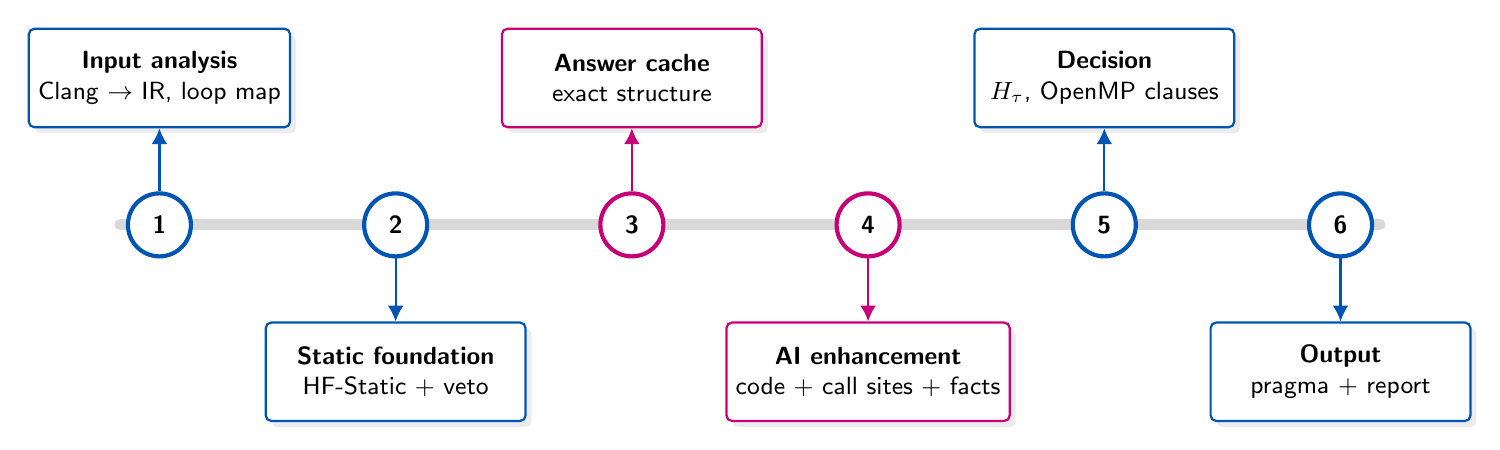
\begin{tikzpicture}[
        node distance=0.5cm and 1.2cm, font=\sffamily\small, >={Latex[length=2mm, width=2mm]},
        process/.style={rectangle, draw=#1, thick, fill=white, minimum width=3.3cm, minimum height=1.25cm,
                        align=center, rounded corners=2pt, drop shadow={opacity=0.15}},
        marker/.style={circle, draw=#1, line width=1.5pt, fill=white, minimum size=0.8cm, inner sep=0pt},
        connector/.style={draw=#1, thick, ->}]
    \draw[gray!30, line width=4pt, line cap=round] (-0.5,0) -- (15.5,0);
    \node[marker=pipelineBlue] (m1) at (0,0) {\textbf{1}};
    \node[process=pipelineBlue, above=0.8cm of m1] (p1) {\textbf{Input analysis}\\Clang $\rightarrow$ IR, loop map};
    \draw[connector=pipelineBlue] (m1) -- (p1);
    \node[marker=pipelineBlue] (m2) at (3,0) {\textbf{2}};
    \node[process=pipelineBlue, below=0.8cm of m2] (p2) {\textbf{Static foundation}\\HF-Static + veto};
    \draw[connector=pipelineBlue] (m2) -- (p2);
    \node[marker=pipelineMagenta] (m3) at (6,0) {\textbf{3}};
    \node[process=pipelineMagenta, above=0.8cm of m3] (p3) {\textbf{Answer cache}\\exact structure};
    \draw[connector=pipelineMagenta] (m3) -- (p3);
    \node[marker=pipelineMagenta] (m4) at (9,0) {\textbf{4}};
    \node[process=pipelineMagenta, below=0.8cm of m4] (p4) {\textbf{AI enhancement}\\code + call sites + facts};
    \draw[connector=pipelineMagenta] (m4) -- (p4);
    \node[marker=pipelineBlue] (m5) at (12,0) {\textbf{5}};
    \node[process=pipelineBlue, above=0.8cm of m5] (p5) {\textbf{Decision}\\$H_\tau$, OpenMP clauses};
    \draw[connector=pipelineBlue] (m5) -- (p5);
    \node[marker=pipelineBlue] (m6) at (15,0) {\textbf{6}};
    \node[process=pipelineBlue, below=0.8cm of m6] (p6) {\textbf{Output}\\pragma + report};
    \draw[connector=pipelineBlue] (m6) -- (p6);
    \end{tikzpicture}}
    \caption{\SystemName{} six-phase pipeline. Blue phases are deterministic; magenta phases involve the language model and are reached only by loops that HF-Static leaves \textsc{Unknown} and that pass the call-site guard.}
    \label{fig:pipeline}
\end{figure}

\subsubsection{Phase 1: Input analysis and loop discovery}
Each translation unit is compiled with Clang to LLVM IR at \Code{-O1} with debug information and with loop unrolling, vectorization and loop-idiom recognition disabled (\Code{-fno-unroll-loops -fno-vectorize -fno-slp-vectorize -mllvm -disable-loop-idiom-all}). This promotes scalars to SSA form, so that inductions and reductions appear as header $\phi$-nodes, while keeping every source loop recognizable and mapped to its source line through the loop's debug location. \Code{loop-simplify} and \Code{lcssa} are run before the analysis. Loops whose debug location lies in a system or library header (e.g.\ STL containers) are discarded, so that only project loops are reported.

\subsubsection{Phase 2: Static foundation and the LLVM veto}
\label{sec:static}
HF-Static is an LLVM~21 new-pass-manager plugin. For every natural loop $L$ (all nesting levels, skipping inlined copies) it evaluates four groups of evidence (Algorithm~\ref{alg:static}) and writes one JSON record with the verdict, every reason, the recognized reductions and the tested dependence pairs.

\begin{algorithm}[htbp]
\caption{HF-Static classification of a loop $L$ at nesting depth $d$}
\label{alg:static}
\footnotesize
\begin{algorithmic}[1]
\STATE $\mathit{Ser} \leftarrow \emptyset$, $\mathit{Unk} \leftarrow \emptyset$
\IF{$L$ has more than one exiting block} \STATE add ``early exit'' to $\mathit{Ser}$ \ENDIF
\IF{SCEV cannot compute the back-edge count} \STATE add ``trip count'' to $\mathit{Unk}$ \ENDIF
\FOR{each header $\phi$-node $p$ of $L$}
  \IF{$p$ is an induction or a recognized reduction} \STATE \textbf{continue} \ENDIF
  \IF{$p$ is only used after $L$} \STATE \textbf{continue} \COMMENT{last value} \ENDIF
  \IF{$p$ forwards a load of memory not written in $L$ whose address does not depend on $p$} \STATE \textbf{continue} \ENDIF
  \IF{the latch value of $p$ is a select/merge that may keep $p$} \STATE add ``conditional scalar update'' to $\mathit{Unk}$
  \ELSE \STATE add ``scalar recurrence'' to $\mathit{Ser}$ \ENDIF
\ENDFOR
\FOR{each call $c$ in $L$}
  \IF{$c$ is order dependent (I/O, \Code{rand})} \STATE add to $\mathit{Ser}$
  \ELSIF{$c$ is not \Code{readnone}, a thread-safe allocation or an errno-only \Code{libm} call} \STATE add to $\mathit{Unk}$ \ENDIF
\ENDFOR
\FOR{each pair $(a,b)$ of memory accesses in $L$, at least one a write}
  \STATE $D \leftarrow \mathrm{DA.depends}(a,b)$
  \IF{$D$ is confused} \STATE add ``inconclusive'' to $\mathit{Unk}$
  \ELSIF{all outer levels admit `$=$' and level $d$ admits `$<$' or `$>$'}
     \IF{the distance at level $d$ is a non-zero constant, or $D$ is consistent with a resolved direction} \STATE add ``proven dependence'' to $\mathit{Ser}$
     \ELSE \STATE add ``possible dependence'' to $\mathit{Unk}$ \ENDIF
  \ENDIF
\ENDFOR
\STATE \textbf{return} \textsc{Serial} if $\mathit{Ser}\neq\emptyset$; else \textsc{Unknown} if $\mathit{Unk}\neq\emptyset$; else \textsc{Parallel} (with the recognized reduction operators)
\end{algorithmic}
\end{algorithm}

Two design choices make the veto safe. First, a dependence is only \emph{proven} when DependenceAnalysis returns a consistent dependence with a resolved non-`$=$' direction or a constant non-zero distance at the loop's own level; everything weaker becomes \textsc{Unknown}, so the veto is never triggered by an imprecise test. Second, \textsc{Parallel} requires the absence of any unresolved evidence. The condition on line~7 (``whose address does not depend on $p$'') was added after the loop-structure extension revealed that a pointer-chasing recurrence (\Code{p = next[p]}) had been accepted as a forwarded load (Section~\ref{sec:rq-ext}); all results in this article use the corrected pass.

\paragraph{Call-site alias guard} HF-Static analyses a function in isolation. A second pass of the plugin inspects every direct call in the same translation unit and reports pairs of pointer arguments that are derived from the same underlying object or that alias analysis cannot separate. An \textsc{Unknown} loop in a function with such a call site receives $\mathit{Safe}(L)=0$ before any model is consulted. The guard is conservative: two disjoint halves of one buffer are also vetoed, a cost we measure in Section~\ref{sec:rq-ext}.

\subsubsection{Phase 3: Structural answer cache}
\label{sec:cachedesign}
To avoid repeated queries for structurally identical code, the source of each queried kernel is tokenized, identifiers are $\alpha$-renamed in order of first occurrence, numeric literals and scalar type names are abstracted, and the token sequence is used as key. A lookup returns the stored answer of the most similar earlier loop if the \Code{difflib} ratio of the token sequences is at least a similarity threshold $s$; $s=1$ means exact structural duplicates only. Section~\ref{sec:rq-cache} quantifies both the savings and the errors this introduces; the deployed configuration uses $s=1$.

\subsubsection{Phase 4: AI enhancement and prompt engineering}
\label{sec:hybrid}
\textsc{Unknown} loops that pass the guard are sent in batches of eight. Each item contains the kernel function with line numbers (the target loop marked), up to three call sites from the same translation unit, and the HF-Static facts: the verdict, the unresolved reasons, recognized reductions, trip-count computability and memory-operation counts. The system prompt states the legality definition of Section~\ref{sec:problem} verbatim and requests a JSON object per loop with a verdict, a confidence in $[0,1]$, the OpenMP clauses and a short reason. We refer to this prompt as \textbf{H}; the LLM-only baseline uses the same instructions without compiler facts (prompt \textbf{P2}). Prompt variants are compared in Section~\ref{sec:rq-prompt}.

\subsubsection{Phases 5--6: Decision and output}
The decision follows Equation~\eqref{eq:hybrid} and is summarized in Algorithm~\ref{alg:hybrid}. $\tau$ is not tuned on the test data: it is chosen on a development split of 30\% of the base kernels as the value with the highest F1-score among those that produce no false positive on that split, and it is then frozen. The output phase emits the directive with the reduction operators found by HF-Static or the clauses returned by the model, together with the reasons for each decision, so that every accepted directive can be audited.

\begin{algorithm}[htbp]
\caption{\SystemName{} decision for a translation unit}
\label{alg:hybrid}
\footnotesize
\begin{algorithmic}[1]
\STATE $R \leftarrow$ HF-Static($\mathcal{L}$); \ $G \leftarrow$ CallSiteGuard(TU)
\STATE $Q \leftarrow \{L \in \mathcal{L} : R[L].\mathit{verdict} = \textsc{Unknown} \wedge \mathit{func}(L) \notin G\}$
\FOR{each batch $B \subseteq Q$ of size 8 not answered by the cache}
  \STATE $A \leftarrow$ ParseJSON(LLM(Prompt$_H$($B$, $R$, call sites))); \ Cache.store($B$, $A$)
\ENDFOR
\FOR{each $L \in \mathcal{L}$}
  \IF{$R[L].\mathit{verdict} = \textsc{Serial}$ \textbf{or} ($R[L].\mathit{verdict}=\textsc{Unknown}$ \textbf{and} $\mathit{func}(L)\in G$)} \STATE $y_L \leftarrow \textsc{Serial}$ \COMMENT{static veto}
  \ELSIF{$R[L].\mathit{verdict} = \textsc{Parallel}$} \STATE $y_L \leftarrow \textsc{Parallel}$ with HF-Static reductions
  \ELSIF{$A[L].v = \textsc{par}$ \textbf{and} $A[L].c \ge \tau$} \STATE $y_L \leftarrow \textsc{Parallel}$ with model clauses
  \ELSE \STATE $y_L \leftarrow \textsc{Serial}$ \COMMENT{unanswered or unparsable $\Rightarrow$ conservative}
  \ENDIF
\ENDFOR
\end{algorithmic}
\end{algorithm}

% ---- end sections/method ----
% ---- begin sections/bench ----
% =======================================================
% 4. BENCHMARKS
% =======================================================
\section{Execution-Validated Loop Benchmarks}
\label{sec:bench}

An evaluation of a parallelization oracle needs labels that do not come from any of the tools being compared. We therefore built two benchmarks whose labels are written under the legality definition of Section~\ref{sec:problem} and then checked by execution, and we keep the 200-file corpus of our preliminary study as an application-scale corpus without labels.

\subsection{HF-LoopBench}
HF-LoopBench is built from \nBenchBases{} hand-written \emph{base kernels}, each a small C function from one of \nBenchDomains{} application domains with exactly one \emph{target loop} and a documented ground-truth (GT) label. The kernels cover the idioms that decide parallelizability in practice: affine DOALL loops and stencils, scalar and array reductions, privatizable and \Code{linear} scalars, gathers through lookup tables or index arrays, disjoint but non-affine writes (bit-manipulated quantum-gate indices, compare-exchange networks, in-place reversals), permutation scatters, and on the serial side flow and anti dependences, scalar recurrences (filters, generators, hash chains), wavefronts, compaction counters, conflicting scatters, order-dependent library calls and early exits.

A generator instantiates every base kernel along three axes: the element type (up to two of \Code{double}, \Code{float}, \Code{int}, \Code{long long}); the data-access form, \textbf{G} (file-scope arrays), \textbf{P} (pointer parameters) or \textbf{R} (\Code{restrict}-qualified parameters); and, for single-input/single-output DOALL and stencil kernels, a \textbf{Q} variant in which the pointer version is \emph{called} with overlapping arguments (\Code{out = buf+1, in = buf}). The Q variant has the same function text as P but is serial, so it can only be classified correctly by looking at the call site. Each instance becomes a function in a domain file together with a test harness that initializes inputs deterministically, calls the kernel once and prints a 64-bit FNV hash of every output array, two order-sensitive sums and the return value. For every file the generator writes the clean source given to all tools (no directives, no labels), an \emph{OpenMP} version with the GT directive on every parallel target loop, and a \emph{race} version with a naive \Code{parallel for} on every canonical serial target loop. Table~\ref{tab:bench} summarizes the result. Instances of one base kernel are correlated, so all confidence intervals are computed with a cluster bootstrap over base kernels and $\tau$ is calibrated on a split by base kernel.
% ---- begin generated/tables/bench ----
% generated by hf/report.py from results/metrics.json - do not edit by hand
\begin{table}[htbp]
\caption{Composition of HF-LoopBench (all numbers counted from the generated sources).}
\label{tab:bench}
\centering
\small
\resizebox{\linewidth}{!}{%
\begin{tabular}{lrrrrrr}
\toprule
Domain & Files & Lines & Base kernels & Target loops & GT par. & GT ser. \\
\midrule
bioinformatics & 2 & 1,018 & 10 & 33 & 21 & 12 \\
climate weather & 3 & 1,840 & 9 & 57 & 42 & 15 \\
cryptography & 2 & 895 & 9 & 29 & 15 & 14 \\
databases & 2 & 1,484 & 11 & 50 & 27 & 23 \\
finance & 3 & 2,256 & 12 & 75 & 42 & 33 \\
geometry graphics & 2 & 1,610 & 8 & 49 & 36 & 13 \\
graph analytics & 2 & 1,647 & 11 & 48 & 27 & 21 \\
image processing & 3 & 2,084 & 12 & 70 & 51 & 19 \\
linear algebra & 4 & 2,749 & 15 & 92 & 66 & 26 \\
machine learning & 4 & 2,787 & 14 & 89 & 66 & 23 \\
medical imaging & 2 & 1,247 & 6 & 38 & 24 & 14 \\
molecular dynamics & 2 & 1,692 & 9 & 51 & 42 & 9 \\
networking & 1 & 787 & 6 & 23 & 9 & 14 \\
quantum simulation & 2 & 1,176 & 6 & 36 & 30 & 6 \\
scientific misc & 3 & 1,727 & 10 & 59 & 42 & 17 \\
signal processing & 4 & 2,663 & 14 & 89 & 54 & 35 \\
sorting searching & 2 & 1,217 & 9 & 39 & 18 & 21 \\
stencil pde & 3 & 1,850 & 10 & 63 & 42 & 21 \\
\textbf{Total} & 46 & 30,729 & 181 & 990 & 654 & 336 \\
\bottomrule
\end{tabular}
}
\end{table}

% ---- end generated/tables/bench ----

\subsection{Dynamic validation of every label}
\label{sec:oracle}
All three versions of every file are compiled with Clang~21 at \Code{-O1 -ffp-contract=off}, so that floating-point evaluation is identical in the serial and OpenMP builds. The OpenMP version is run with 2, 4 and 8 threads under the schedules \Code{static}, \Code{static,1}, \Code{dynamic,1} and \Code{guided} (12 runs); a parallel label is accepted only if every run reproduces the serial output (bit-exact hash, or relative tolerance $10^{-8}$/$10^{-3}$ on the sums for \Code{double}/\Code{float} reductions). The race version is run with 4 and 8 threads under \Code{static,1} and \Code{dynamic,1}, three times each; a canonical serial label is \emph{confirmed} if at least one run deviates. Table~\ref{tab:oracle} shows the outcome: no parallel label was violated, and every canonical serial label of HF-LoopBench produced a wrong result under naive parallelization.
% ---- begin generated/tables/oracle ----
% generated by hf/report.py from results/metrics.json - do not edit by hand
\begin{table}[htbp]
\caption{Dynamic validation of the ground truth on the M1 Pro.}
\label{tab:oracle}
\centering
\small
\begin{tabular}{lr}
\toprule
Outcome & Loops \\
\midrule
GT-parallel loops verified (12 runs each) & 654 \\
GT-parallel loops violating their label & 0 \\
GT-serial loops whose naive parallelisation changed the output & 321 \\
GT-serial loops without an observed deviation & 0 \\
GT-serial loops not in OpenMP canonical form & 15 \\
\bottomrule
\end{tabular}
\end{table}

% ---- end generated/tables/oracle ----

The harness also exposed a toolchain defect. At \Code{-O2}, the Homebrew build of Clang~21.1.1 produced wrong results for integer whole-array and array-section reductions even with a single thread (in a 15-line reproducer, \Code{hist[px[i]]++} with \Code{reduction(+:hist)} lost about 0.6\% of the increments at \Code{-O2} and \Code{-O3}, already with a single thread, while \Code{-O1}, \Code{-O0} and \Code{-O2 -fno-vectorize} were correct). The oracle therefore uses \Code{-O1}; in the \Code{-O2} performance build of Section~\ref{sec:rq-perf}, the \nPerfMismatch{} affected kernels---all integer array reductions---are excluded from the speedup statistics. The episode illustrates why a proposed directive, whether produced by a compiler, a model or a human, should be validated by differential execution before it is merged.

\subsection{HF-LoopBench-X: a loop-structure extension}
\label{sec:benchx}
HF-LoopBench is organized by application domain and dependence class. To test whether the conclusions carry over to loop \emph{shapes} that it covers thinly, we wrote \xBases{} further base kernels \emph{after} all rules, prompts and thresholds of the main study had been frozen. They include three \emph{level pairs} whose loop nest is textually identical but whose target loop differs (the spatial loop inside a time-step loop is parallel, the time-step loop itself is not; a column loop inside a vertical accumulation is parallel, the level loop is not; a row-diffusion versus a wavefront update of the same grid); triangular nests; stride-2 and step-4 loops; decrementing loops; an unsigned induction variable; walking-pointer loops (\Code{*q++ = *p++ * s}, legal with \Code{linear(p,q:1)}); \Code{collapse(2)}; if/else, masked and \Code{continue} bodies; product and nested reductions; a privatizable temporary array; disjoint in-place updates (a stride-7 modulo interleaver over a power-of-two buffer, a half-buffer shift, pair swaps, a permuted update); and subtle serial loops (a cross-statement flow dependence, a distance-2 recurrence, an anti dependence with a run-time offset, a conditional recurrence, an 8-slot ring buffer, an arg-min, a linked-list walk). Besides the overlapping-call variant Q, every eligible kernel also gets a variant \textbf{H} that is called with two \emph{disjoint} halves of one buffer and therefore remains parallel; it measures how often the conservative call-site guard vetoes a legal loop. The generator, harness and oracle are those of HF-LoopBench. Of the \xLoops{} target loops (\xPar{} parallel, \xSer{} serial), all \xVerified{} parallel labels were verified and \xManifested{} serial labels produced a deviation; the remaining \xNotManifested{} are the arg-min loop, which is serial under our definition because OpenMP has no built-in reduction that returns both the minimum and its index, but whose race did not change the result in 12 runs.

\subsection{Application-scale corpus}
The 200 C++ files (\fieldLines{} lines) of our preliminary study---trading, computer vision, cryptography, finance, healthcare, machine learning, networking, quantum computing, scientific computing and weather/climate code using classes, STL containers and helper functions---have no ground truth. We use them to measure how HF-Static scales and how many loops of realistic code would be routed to the model (Section~\ref{sec:rq-field}).

% ---- end sections/bench ----
% ---- begin sections/setup ----
% =======================================================
% 5. EXPERIMENTAL SETUP
% =======================================================
\section{Experimental Setup}
\label{sec:setup}

\paragraph{Platform} All compilation, analysis, validation and timing were performed on one Apple MacBook Pro with an Apple M1 Pro (\nCpuCores{} cores: \nPerfCores{} performance + \nEffCores{} efficiency), 16\,GB of memory and macOS \macosVersion{}, using Homebrew LLVM/Clang \llvmVersion{} with its bundled OpenMP runtime and Polly. Homebrew GCC~12.2 cannot compile against the macOS~26 SDK headers, so the GCC baseline was run with \gccVersion{} in an Ubuntu 22.04 virtual machine on the same computer; it is a compile-time analysis whose result does not depend on the host. Language models were accessed through the Groq API on 15 and 17 November 2026. The Llama~3.3~70B model used in our preliminary version is no longer served by that provider (the model list returned on 17 November 2026 contains only the three models below among general-purpose chat models), so it could not be re-evaluated.

\paragraph{Research questions}
\begin{description}
  \item[RQ1] How precise and complete is a sound compiler analysis (HF-Static, GCC, Polly) under an execution-validated ground truth?
  \item[RQ2] How reliable are LLMs as stand-alone parallelism oracles, and which loops do they get wrong?
  \item[RQ3] Does the hybrid procedure recover the opportunities the compiler misses without introducing unsafe directives, how does $\tau$ govern this trade-off, and do the results hold on all loops and on loop shapes written after the study was frozen?
  \item[RQ4] What do the pipeline, its cache and the prompt design cost, and how sensitive are the results to the prompt, the model and repeated runs?
  \item[RQ5] What run-time benefit do the parallelized loops deliver, and how does the pipeline behave on application-scale code?
\end{description}

\paragraph{Tools}
\textit{LLVM-only (HF-Static)} is the pass of Section~\ref{sec:static}; used alone it treats \textsc{Unknown} as serial.
\textit{GCC autopar}: \Code{gcc -O2 -ftree-parallelize-loops=8 --param parloops-min-per-thread=2 -fopt-info-loop-optimized}; a target loop counts as parallel if GCC reports ``parallelizing (outer|inner) loop'' at its header line. The low \Code{min-per-thread} value removes GCC's profitability filter so that legality, not profitability, is measured.
\textit{Polly}: \Code{clang -O3 -mllvm -polly -mllvm -polly-parallel -mllvm -polly-process-unprofitable}; a target loop counts as parallel if Polly outlines a parallel sub-function that covers it and is not launched from inside an enclosing loop.
\textit{AI-only}: \Code{openai/gpt-oss-120b} and \Code{openai/gpt-oss-20b} with reasoning effort ``low'' and JSON mode, and \Code{qwen/qwen3.8-27b} without reasoning, all at temperature~0 with a fixed seed, prompt P2, verdict \textsc{par} counted as parallel.
\textit{Hybrid}: Algorithm~\ref{alg:hybrid} with prompt H. Every request and raw response is appended to a log; re-running an experiment replays the log instead of calling the API.

\paragraph{Evaluation sets and API limits} On the free API tier the rate-limit headers reported 8{,}000 tokens per minute for each of the three models; Qwen3.8-27B was in addition limited to 1{,}000 output tokens per minute and, according to the provider's error message, 200{,}000 tokens per day. These limits shaped the design of the LLM experiments: the Qwen repetition run was stopped by the daily limit on 15 November after 88 of 120 loops and completed on 17 November from the replay log, without re-issuing the answered requests. The compiler tools are evaluated on all \nBenchLoops{} loops. The AI-only baseline and the threshold calibration use an \emph{evaluation set} of \nEvalLoops{} loops (one element type per base kernel and the access forms G, P and Q); HF-Static is \textsc{Unknown} for \nEvalUnknown{} of them. The remaining \textsc{Unknown} loops of HF-LoopBench (second element type and \Code{restrict} variants) were later answered with prompt H at the frozen threshold, so that the complete pipeline can be scored on all loops (Section~\ref{sec:rq-full}). On HF-LoopBench-X every loop is evaluated. The prompt ablation uses a fixed subset of \nAblLoops{} loops (one instance per base kernel, G or P form).

\paragraph{Prompts} \textbf{P1} asks in one sentence whether each loop can be parallelized with \Code{parallel for} and imposes no output format. \textbf{P2} states the legality definition and a JSON schema. \textbf{P3} adds two worked examples and asks for an explicit dependence analysis before the verdict. \textbf{P4} adds a digest of the OpenMP~5.2 rules that decide legality (canonical loop form, data-sharing defaults, reduction and \Code{linear} semantics, order independence, pointer overlap). \textbf{H} is P2 plus the HF-Static facts. All prompts are released with the artifact.

\paragraph{Metrics and statistics} The positive class is \textsc{Parallel}. We report TP, FP, TN, FN, precision, recall, F1 and the Matthews correlation coefficient (MCC). 95\% confidence intervals use a cluster bootstrap over base kernels (2{,}000 resamples). Paired comparisons use the exact McNemar test on per-loop correctness, which---unlike a $t$-test over a single run---needs no distributional assumption and respects the pairing of methods on the same loops. Run-to-run consistency is measured with Cohen's $\kappa$ between two independent runs of the same prompt. $\tau$ is selected per model on a development split containing 30\% of the base kernels (chosen by a hash of the kernel name) and results are also reported on the disjoint 70\% test split. Per-class, cache and cost analyses use one \emph{primary} model, the one whose complete hybrid configuration has the highest F1-score on the development split (GPT-OSS-20B).

% ---- end sections/setup ----
% ---- begin sections/results ----
% =======================================================
% 6. RESULTS
% =======================================================
\section{Results and Detailed Analysis}
\label{sec:results}

\subsection{Pipeline reduction on application-scale code}
\label{sec:rq-field}
Table~\ref{tab:pipeline} follows the loops of the 200-file corpus through the deterministic phases. Phase~1 finds \plRaw{} natural loops, of which \plHeader{} lie in system and library headers (mostly STL containers) and are discarded. Of the remaining \fieldLoops{} project loops, HF-Static decides \plDecided{} (\plDecidedPct{}) without any model: \fieldPar{} are proven parallel and \fieldSer{} serial, the most frequent serial reasons being early exits (\Code{break}/\Code{return}) and scalar recurrences. The \fieldUnk{} \textsc{Unknown} loops (\fieldPctUnk{}) are the population on which the hybrid procedure operates; their most frequent reasons are unresolved dependence directions and calls with unknown side effects (often STL member functions). The whole corpus is analysed in \fieldSeconds{}\,s, of which the pass itself takes \plPassSeconds{}\,s; the rest is IR generation.
% ---- begin generated/tables/pipeline ----
% generated by hf/paper_extra.py - do not edit by hand

\begin{table}[htbp]
\caption{Loops of the 200-file application corpus (37,719 lines, 10 domains) through the deterministic phases.}
\label{tab:pipeline}
\centering
\small
\begin{tabular}{lrr}
\toprule
Pipeline phase & Loops & Share \\
\midrule
Phase 1: natural loops found (incl.\ system/library headers) & 2,187 &  \\
Phase 1: loops in system/library headers removed & $-$343 &  \\
Phase 1: project loops & 1,844 & 100.0\% \\
\midrule
Phase 2: proven \textsc{Parallel} (directive emitted, no model call) & 303 & 16.4\% \\
Phase 2: proven \textsc{Serial} (veto) & 592 & 32.1\% \\
Phase 2: \textsc{Unknown} $\rightarrow$ candidates for Phases 3--4 & \textbf{949} & \textbf{51.5\%} \\
\bottomrule
\end{tabular}
\end{table}

% ---- end generated/tables/pipeline ----

\subsection{RQ1: The LLVM-only baseline under an execution-validated ground truth}
\label{sec:rq-static}
Table~\ref{tab:fullset} compares the three sound compiler tools on all \nBenchLoops{} loops of HF-LoopBench.
% ---- begin generated/tables/fullset ----
% generated by hf/report.py from results/metrics.json - do not edit by hand
\begin{table}[htbp]
\caption{Compiler-based tools on all 990 target loops (95\% cluster-bootstrap CI).}
\label{tab:fullset}
\centering
\small
\resizebox{\linewidth}{!}{%
\begin{tabular}{lrrrrrrrr}
\toprule
Tool & TP & FP & TN & FN & Prec. & Rec. & F1 [95\% CI] & MCC \\
\midrule
HF-Static (LLVM 21) & 377 & 2 & 334 & 277 & 99.5 & 57.6 & 73.0 [67.7, 77.9] & 0.556 \\
GCC autopar & 233 & 0 & 336 & 421 & 100.0 & 35.6 & 52.5 [44.9, 59.9] & 0.398 \\
Polly & 66 & 7 & 329 & 588 & 90.4 & 10.1 & 18.2 [9.0, 27.1] & 0.145 \\
\bottomrule
\end{tabular}
}
\end{table}

% ---- end generated/tables/fullset ----

HF-Static decides \nStaticSertoSer{} of the \nBenchSer{} serial loops correctly as \textsc{Serial} and accepts \fsStaticTP{} of the \nBenchPar{} parallel loops (precision \fsStaticPrec{}, recall \fsStaticRec{}, F1 \fsStaticFone{}). GCC is equally conservative but finds fewer loops (recall \fsGccRec{}), and Polly parallelizes only \fsPollyTP{} target loops because most kernels are not static control parts. The \nStaticFalsePar{} serial loops that HF-Static labels \textsc{Parallel} are the \Code{restrict} variants of a kernel that stages every element through a caller-provided scratch cell (\Code{*scratch = a[i]*2; b[i] = *scratch + 1;}): with \Code{restrict}, LLVM promotes the scratch cell to a register before the analysis runs, so the IR loop is genuinely independent, but no OpenMP clause can privatize \Code{*scratch} at source level. This is a limitation of IR-level analysis for source-level directives rather than of dependence testing. Polly's \fsPollyFP{} ``false positives'' fall outside our directive-only definition: six are variants of a column-wise integral-image nest that Polly parallelizes after transforming the nest, and one is an overlapping-argument variant, for which Polly emits code versioned on run-time alias checks.

The price of soundness is the \textsc{Unknown} class: \nStaticPartoUnk{} parallel and \nStaticSertoUnk{} serial loops are left undecided. The recorded reasons (Table~\ref{tab:unknown}) are dominated by pointer parameters that alias analysis cannot separate and by flattened multi-dimensional subscripts (\Code{a[i*m+j]}) for which DependenceAnalysis cannot resolve the direction at the outer level. The pass needs \staticUsPerLoop{}\,\textmu s per loop on average. In short, the LLVM-only configuration is safe but finds little more than half of the parallelism; the 96.6\% F1 of our preliminary version was an artefact of using the pass as its own oracle.

\begin{table}[htbp]
\caption{Reasons recorded by HF-Static for \textsc{Unknown} target loops of HF-LoopBench (a loop can have several).}
\label{tab:unknown}
\centering\small
% ---- begin generated/tables/unknown_reasons_body ----
% generated by hf/report.py
\begin{tabular}{lr}
\toprule
Reason reported by HF-Static & Loops \\
\midrule
dependence test inconclusive (may-alias or non-affine subscript) & 213 \\
possible loop-carried output dependence (direction not resolved) & 206 \\
possible loop-carried anti dependence (direction not resolved) & 159 \\
conditionally updated scalar (possible min/max/last-value reduction) & 75 \\
possible loop-carried flow dependence (direction not resolved) & 24 \\
\bottomrule
\end{tabular}

% ---- end generated/tables/unknown_reasons_body ----
\end{table}

\subsection{RQ2: LLMs alone and the hallucination problem}
\label{sec:rq-ai}
Table~\ref{tab:evalset} lists all methods on the \nEvalLoops{}-loop evaluation set. Contrary to our preliminary version, current open-weight models are \emph{strong} classifiers when used alone: with prompt P2, GPT-OSS-120B reaches F1 \evAIOneTwentyFone{} and GPT-OSS-20B \evAITwentyFone{}, well above HF-Static (\evStaticFone{}) on the same loops, because they recognize stencils, gathers, privatizable temporaries and pointer-parameter DOALL loops that the compiler cannot prove.
% ---- begin generated/tables/evalset ----
% generated by hf/report.py from results/metrics.json - do not edit by hand
\begin{table}[htbp]
\caption{All methods on the LLM evaluation set (396 loops).}
\label{tab:evalset}
\centering
\small
\resizebox{\linewidth}{!}{%
\begin{tabular}{lrrrrrrrr}
\toprule
Method & TP & FP & TN & FN & Prec. & Rec. & F1 [95\% CI] & MCC \\
\midrule
HF-Static (LLVM 21) & 115 & 0 & 154 & 127 & 100.0 & 47.5 & 64.4 [58.8, 69.6] & 0.510 \\
GCC autopar & 73 & 0 & 154 & 169 & 100.0 & 30.2 & 46.3 [39.2, 53.2] & 0.379 \\
Polly & 24 & 3 & 151 & 218 & 88.9 & 9.9 & 17.8 [9.0, 26.3] & 0.154 \\
AI-only GPT-OSS-120B & 219 & 38 & 116 & 23 & 85.2 & 90.5 & 87.8 [84.6, 90.6] & 0.672 \\
Hybrid GPT-OSS-120B, no facts ($\tau^*$) & 215 & 2 & 152 & 27 & 99.1 & 88.8 & 93.7 [90.5, 96.4] & 0.858 \\
Hybrid GPT-OSS-120B, no call-site guard ($\tau^*$) & 136 & 7 & 147 & 106 & 95.1 & 56.2 & 70.6 [65.1, 75.9] & 0.524 \\
Hybrid GPT-OSS-120B ($\tau{=}0.5$) & 217 & 2 & 152 & 25 & 99.1 & 89.7 & 94.1 [91.1, 96.7] & 0.866 \\
Hybrid GPT-OSS-120B ($\tau^*$) & 136 & 0 & 154 & 106 & 100.0 & 56.2 & 72.0 [66.3, 77.1] & 0.577 \\
AI-only GPT-OSS-20B & 202 & 43 & 111 & 40 & 82.4 & 83.5 & 83.0 [79.2, 86.4] & 0.558 \\
Hybrid GPT-OSS-20B, no facts ($\tau^*$) & 212 & 5 & 149 & 30 & 97.7 & 87.6 & 92.4 [88.7, 95.4] & 0.826 \\
Hybrid GPT-OSS-20B, no call-site guard ($\tau^*$) & 209 & 34 & 120 & 33 & 86.0 & 86.4 & 86.2 [82.6, 89.4] & 0.644 \\
Hybrid GPT-OSS-20B ($\tau{=}0.5$) & 209 & 0 & 154 & 33 & 100.0 & 86.4 & 92.7 [89.1, 95.8] & 0.843 \\
Hybrid GPT-OSS-20B ($\tau^*$) & 209 & 0 & 154 & 33 & 100.0 & 86.4 & 92.7 [89.1, 95.8] & 0.843 \\
\bottomrule
\end{tabular}
}
\end{table}

% ---- end generated/tables/evalset ----

They are, however, not safe. GPT-OSS-120B declares \evAIOneTwentyFP{} serial loops parallel and GPT-OSS-20B \evAITwentyFP{} (precision \evAIOneTwentyPrec{} and \evAITwentyPrec{}); each of these would be a data race. For the primary model, \nAIFPQ{} of the unsafe answers concern the overlapping-call variants: the function body is a textbook DOALL loop, the call site printed in the prompt (\Code{f(buf + 1, buf, n)}) makes it serial, and the model's explanation (``each iteration writes distinct \Code{y[i]}'') shows that the call site was ignored. The remaining \nAIFPnonQ{} are loop-carried flow dependences and scalar recurrences that were misread, a conflicting scatter and the shared scratch cell.

Table~\ref{tab:aidist} breaks the model's answers down by self-reported confidence. Most answers, correct or not, carry a confidence of at least 0.95, and every one of the \aiUnsafeTwenty{} unsafe answers of GPT-OSS-20B (\aiHiConfUnsafeOneTwenty{} of \aiUnsafeOneTwenty{} for GPT-OSS-120B) was given with a confidence of at least 0.9. Confidence therefore separates correct from incorrect answers only weakly, which limits what a threshold alone can achieve (Section~\ref{sec:rq-tau}). On the other side, both models systematically reject histogram-style array reductions (\Code{hist[px[i]]++}) that \Code{reduction(+:hist[:256])} makes legal (Section~\ref{sec:case-hist}).
% ---- begin generated/tables/ai_dist ----
% generated by hf/paper_extra.py - do not edit by hand

\begin{table}[htbp]
\caption{Answers of the LLMs alone (prompt P2, evaluation set) by self-reported confidence $c$. Unsafe: ``parallel'' answers for loops whose GT is serial; missed: ``serial'' answers for GT-parallel loops.}
\label{tab:aidist}
\centering
\small
\resizebox{\linewidth}{!}{%
\begin{tabular}{lrrrrrrrr}
\toprule
 & \multicolumn{4}{c}{GPT-OSS-20B} & \multicolumn{4}{c}{GPT-OSS-120B} \\ Confidence & ``parallel'' & unsafe & ``serial'' & missed & ``parallel'' & unsafe & ``serial'' & missed \\
\midrule
$c \ge 0.95$ & 245 & 43 & 145 & 37 & 251 & 38 & 136 & 22 \\
$0.90 \le c < 0.95$ & 0 & 0 & 5 & 2 & 6 & 0 & 3 & 1 \\
$0.80 \le c < 0.90$ & 0 & 0 & 1 & 1 & 0 & 0 & 0 & 0 \\
$c < 0.80$ & 0 & 0 & 0 & 0 & 0 & 0 & 0 & 0 \\
no parsable answer & 0 &  &  &  & 0 &  &  &  \\
\bottomrule
\end{tabular}
}
\end{table}

% ---- end generated/tables/ai_dist ----

\subsection{RQ3: The hybrid procedure}
\label{sec:rq-hybrid}

\paragraph{Static veto} In the hybrid pipeline the model is asked only about the \nEvalUnknown{} \textsc{Unknown} loops of the evaluation set; every other decision comes from HF-Static. This removes all unsafe answers on loops with a proven dependence: for the primary model the veto overrides \nVetoSaves{} unsafe answers directly. It cannot remove the overlapping-call variants, for which HF-Static analyses the callee in isolation and reports \textsc{Unknown}: without a further guard, the hybrid with GPT-OSS-20B still emits \evHTwentyFP{} unsafe directives (row ``no call-site guard'' in Table~\ref{tab:evalset}), all of them on these loops.

\paragraph{Call-site guard} With the guard of Section~\ref{sec:static}, which flags exactly the \nCtxFlaggedAll{} overlapping-call instances of HF-LoopBench and no other kernel, the complete hybrid with GPT-OSS-20B ($\tau^*=\tauStarTwenty$) accepts \evHCTwentyTP{} of the \nEvalPar{} parallel loops of the evaluation set without a single unsafe directive (precision \evHCTwentyPrec{}, recall \evHCTwentyRec{}, F1 \evHCTwentyFone{} [\evHCTwentyFoneLo{}, \evHCTwentyFoneHi{}], MCC \evHCTwentyMCC{}); on the held-out 70\% test split the F1 is \evHCTwentyTestFone{} with \evHCTwentyTestFP{} false positives. Compared with the LLVM-only baseline, recall rises from \evStaticRec{} to \evHCTwentyRec{} at unchanged precision; compared with the LLM alone, all \evAITwentyFP{} unsafe answers disappear and F1 rises from \evAITwentyFone{} to \evHCTwentyFone{}.

\paragraph{Effect of the compiler facts} The row ``no facts'' answers the \textsc{Unknown} loops with the P2 answers (no compiler facts) under the same veto and guard. For GPT-OSS-20B the facts remove the \evHBTwentyFP{} unsafe answers that remain without them at a similar recall (\evHCTwentyRec{} vs.\ \evHBTwentyRec{}). For GPT-OSS-120B they do not help: the facts lower the confidence the model reports, so that at its calibrated threshold the complete system accepts fewer loops (F1 \evHCOneTwentyFone{}) than the no-facts variant (F1 \evHBOneTwentyFone{}, \evHBOneTwentyFP{} unsafe directives). Injecting compiler facts is therefore not uniformly beneficial; what makes the pipeline safe is the veto and the guard, and the threshold must be calibrated per model and prompt.

\subsubsection{Statistical significance}
Table~\ref{tab:mcnemar} reports exact McNemar tests on per-loop correctness. The complete hybrid is significantly more often correct than both single-modality baselines for both models ($p<0.001$); for GPT-OSS-20B there is no loop on which the LLVM-only baseline is correct and the hybrid is not.
% ---- begin generated/tables/mcnemar ----
% generated by hf/paper_extra.py - do not edit by hand

\begin{table}[htbp]
\caption{Exact McNemar tests on per-loop correctness (evaluation set, 396 loops). $b$: loops only the first method gets right; $c$: loops only the second gets right.}
\label{tab:mcnemar}
\centering
\footnotesize
\begin{tabular}{lrrr}
\toprule
Comparison & $b$ & $c$ & $p$ \\
\midrule
Hybrid GPT-OSS-120B vs.\ AI-only GPT-OSS-120B & 40 & 85 & $<0.001$ \\
Hybrid GPT-OSS-120B vs.\ LLVM-only & 21 & 0 & $<0.001$ \\
Hybrid GPT-OSS-120B vs.\ Hybrid GPT-OSS-120B w/o guard & 7 & 0 & 0.016 \\
AI-only GPT-OSS-120B vs.\ LLVM-only & 106 & 40 & $<0.001$ \\
Hybrid GPT-OSS-120B vs.\ Hybrid GPT-OSS-120B w/o facts & 2 & 79 & $<0.001$ \\
Hybrid GPT-OSS-120B vs.\ GCC & 67 & 4 & $<0.001$ \\
Hybrid GPT-OSS-20B vs.\ AI-only GPT-OSS-20B & 57 & 7 & $<0.001$ \\
Hybrid GPT-OSS-20B vs.\ LLVM-only & 94 & 0 & $<0.001$ \\
Hybrid GPT-OSS-20B vs.\ Hybrid GPT-OSS-20B w/o guard & 34 & 0 & $<0.001$ \\
AI-only GPT-OSS-20B vs.\ LLVM-only & 97 & 53 & $<0.001$ \\
Hybrid GPT-OSS-20B vs.\ Hybrid GPT-OSS-20B w/o facts & 9 & 7 & 0.804 \\
Hybrid GPT-OSS-20B vs.\ GCC & 136 & 0 & $<0.001$ \\
\bottomrule
\end{tabular}
\end{table}

% ---- end generated/tables/mcnemar ----

\subsubsection{Confidence-threshold sensitivity (\texorpdfstring{$\tau$}{tau})}
\label{sec:rq-tau}
The threshold lets a user govern the model's influence (Tables~\ref{tab:sweep-gpt-oss-20b} and~\ref{tab:sweep-gpt-oss-120b}). For GPT-OSS-20B the complete system is already safe at $\tau=0.5$ on the development split, so calibration selects $\tau^*=\tauStarTwenty$; raising $\tau$ only costs recall (F1 \swHCFoneNinetyFiveTwenty{} at 0.95). For GPT-OSS-120B the development split contains one serial loop---an in-place running maximum, \Code{img[i] = max(img[i-1], img[i])}---that the model calls parallel with confidence 0.9, so calibration selects $\tau^*=\tauStarOneTwenty$: the system becomes safe (\evHCOneTwentyFP{} unsafe directives) but its F1 drops to \evHCOneTwentyFone{}, whereas $\tau=0.5$ would give F1 \evHFiftyOneTwentyFone{} with \evHFiftyOneTwentyFP{} unsafe directives. As in our preliminary version, a high threshold buys safety; unlike in that version, the value is chosen on held-out kernels and its cost in recall is reported. The larger model is the better stand-alone classifier but the worse partner in the hybrid: its errors are confident, and confidence is the only signal the gate can use.
% ---- begin generated/tables/sweep_gpt-oss-20b ----
% generated by hf/report.py from results/metrics.json - do not edit by hand
\begin{table}[htbp]
\caption{Sensitivity to the confidence threshold $\tau$ (openai/gpt-oss-20b).}
\label{tab:sweep-gpt-oss-20b}
\centering
\small
\resizebox{\linewidth}{!}{%
\begin{tabular}{rrrrrrrrrrr}
\toprule
$\tau$ & AI-only FP & AI-only F1 & No facts FP & No facts F1 & No guard FP & No guard F1 & Full TP & Full FP & Full F1 & Full FP (dev) \\
\midrule
0.50 & 43 & 83.0 & 5 & 92.4 & 34 & 86.2 & 209 & 0 & 92.7 & 0 \\
0.60 & 43 & 83.0 & 5 & 92.4 & 34 & 86.2 & 209 & 0 & 92.7 & 0 \\
0.70 & 43 & 83.0 & 5 & 92.4 & 34 & 86.2 & 209 & 0 & 92.7 & 0 \\
0.80 & 43 & 83.0 & 5 & 92.4 & 34 & 86.2 & 209 & 0 & 92.7 & 0 \\
0.85 & 43 & 83.0 & 5 & 92.4 & 34 & 86.0 & 208 & 0 & 92.4 & 0 \\
0.90 & 43 & 83.0 & 5 & 92.4 & 31 & 84.6 & 200 & 0 & 90.5 & 0 \\
0.95 & 43 & 83.0 & 5 & 92.4 & 16 & 77.1 & 162 & 0 & 80.2 & 0 \\
0.99 & 33 & 68.7 & 3 & 85.2 & 4 & 66.3 & 122 & 0 & 67.0 & 0 \\
\bottomrule
\end{tabular}
}
\par\smallskip\footnotesize AI-only: P2 answers gated by $\tau$. No facts: veto + call-site guard + P2 answers. No guard: veto + H answers. Full: veto + call-site guard + H answers (complete system). F1 in \%.
\end{table}

% ---- end generated/tables/sweep_gpt-oss-20b ----
% ---- begin generated/tables/sweep_gpt-oss-120b ----
% generated by hf/report.py from results/metrics.json - do not edit by hand
\begin{table}[htbp]
\caption{Sensitivity to the confidence threshold $\tau$ (openai/gpt-oss-120b).}
\label{tab:sweep-gpt-oss-120b}
\centering
\small
\resizebox{\linewidth}{!}{%
\begin{tabular}{rrrrrrrrrrr}
\toprule
$\tau$ & AI-only FP & AI-only F1 & No facts FP & No facts F1 & No guard FP & No guard F1 & Full TP & Full FP & Full F1 & Full FP (dev) \\
\midrule
0.50 & 38 & 87.8 & 2 & 95.1 & 37 & 87.5 & 217 & 2 & 94.1 & 1 \\
0.60 & 38 & 87.8 & 2 & 95.1 & 37 & 87.5 & 217 & 2 & 94.1 & 1 \\
0.70 & 38 & 87.8 & 2 & 95.1 & 37 & 87.0 & 215 & 2 & 93.7 & 1 \\
0.80 & 38 & 87.8 & 2 & 95.1 & 37 & 85.9 & 210 & 2 & 92.5 & 1 \\
0.85 & 38 & 87.8 & 2 & 95.1 & 35 & 84.8 & 204 & 1 & 91.3 & 1 \\
0.90 & 38 & 87.8 & 2 & 95.1 & 28 & 82.9 & 191 & 1 & 88.0 & 1 \\
0.95 & 38 & 86.4 & 2 & 93.7 & 7 & 70.6 & 136 & 0 & 72.0 & 0 \\
0.99 & 30 & 74.9 & 0 & 87.7 & 0 & 64.4 & 115 & 0 & 64.4 & 0 \\
\bottomrule
\end{tabular}
}
\par\smallskip\footnotesize AI-only: P2 answers gated by $\tau$. No facts: veto + call-site guard + P2 answers. No guard: veto + H answers. Full: veto + call-site guard + H answers (complete system). F1 in \%.
\end{table}

% ---- end generated/tables/sweep_gpt-oss-120b ----

\subsubsection{All loops of HF-LoopBench}
\label{sec:rq-full}
The evaluation set contains one element type and no \Code{restrict} variant per kernel. To score the complete pipeline on the whole benchmark, the remaining \textsc{Unknown} loops were answered later with prompt H at the frozen thresholds. Table~\ref{tab:fullhybrid} compares the result with the compiler tools on all \nBenchLoops{} loops. With GPT-OSS-20B the hybrid accepts \fhTwentyTP{} of the \nBenchPar{} parallel loops (recall \fhTwentyRec{}, F1 \fhTwentyFone{} [\fhTwentyFoneLo{}, \fhTwentyFoneHi{}]) with \fhTwentyFP{} unsafe directives\fhTwentyFPNote{} Two of them are the \Code{restrict} scratch-cell loops that HF-Static itself accepts (Section~\ref{sec:rq-static}); the other two are \Code{float} variants of a Bellman--Ford relaxation and of a time-stepping loop for which the model answered ``parallel'' with confidence 0.9, although it had answered ``serial'' with confidence 0.85--0.99 for the textually equivalent \Code{double} variants of the same kernels. The model is thus not even consistent across element types, which no threshold calibrated on other loops can anticipate. On the \fhOutN{} loops outside the evaluation set, which played no role in calibration, the hybrid's F1 is \fhTwentyOutFone{} against \fhStaticOutFone{} for HF-Static. With GPT-OSS-120B at its conservative $\tau^*$ the hybrid reaches F1 \fhOneTwentyFone{} with \fhOneTwentyFP{} unsafe directives (both the scratch-cell loops), whereas $\tau=0.5$ would give \fhOneTwentyFiftyFone{} with \fhOneTwentyFiftyFP{}. The model was queried for \fhTwentyQueried{} of the \nBenchLoops{} loops (\fhQueriedPct{}).
% ---- begin generated/tables/fullhybrid ----
% generated by hf/paper_extra.py - do not edit by hand

\begin{table}[htbp]
\caption{All 990 loops of HF-LoopBench: sound compiler tools versus the complete hybrid (thresholds frozen at the values calibrated on the evaluation set's development split).}
\label{tab:fullhybrid}
\centering
\small
\resizebox{\linewidth}{!}{%
\begin{tabular}{lrrrrrrrr}
\toprule
Method & TP & FP & TN & FN & Prec. & Rec. & F1 [95\% CI] & MCC \\
\midrule
LLVM-only (HF-Static) & 377 & 2 & 334 & 277 & 99.5 & 57.6 & 73.0 [67.7, 77.9] & 0.556 \\
GCC autopar & 233 & 0 & 336 & 421 & 100.0 & 35.6 & 52.5 [44.9, 59.9] & 0.398 \\
Polly & 66 & 7 & 329 & 588 & 90.4 & 10.1 & 18.2 [9.0, 27.1] & 0.145 \\
Hybrid GPT-OSS-120B ($\tau{=}0.5$) & 577 & 8 & 328 & 77 & 98.6 & 88.2 & 93.1 & 0.827 \\
\textbf{Hybrid GPT-OSS-120B} ($\tau^*{=}0.95$) & 411 & 2 & 334 & 243 & 99.5 & 62.8 & 77.0 [72.2, 81.7] & 0.598 \\
Hybrid GPT-OSS-20B ($\tau{=}0.5$) & 566 & 4 & 332 & 88 & 99.3 & 86.5 & 92.5 & 0.818 \\
\textbf{Hybrid GPT-OSS-20B} ($\tau^*{=}0.5$) & 566 & 4 & 332 & 88 & 99.3 & 86.5 & 92.5 [89.0, 95.5] & 0.818 \\
\bottomrule
\end{tabular}
}
\end{table}

% ---- end generated/tables/fullhybrid ----

\subsubsection{Loop-structure extension (HF-LoopBench-X)}
\label{sec:rq-ext}
Table~\ref{tab:ext} reports all methods on the \xLoops{} loops of HF-LoopBench-X, with every hybrid threshold frozen at the value calibrated on HF-LoopBench, and Table~\ref{tab:ext-classes} breaks the results down by loop structure. \extText{}

The two unsafe directives of the GPT-OSS-20B hybrid are the global and pointer variants of \Code{for (i = 0; i < n - k; i++) a[i] = a[i + k] * c;}, an anti dependence whose distance \Code{k} is a run-time parameter (3 at the only call site). HF-Static cannot resolve the direction of a symbolic distance and reports \textsc{Unknown}; the model answered ``parallel'' with confidence 0.9 and 0.95 (``each iteration writes distinct \Code{a[i]} and reads \Code{a[i+k]}''), while it answered ``serial'' for the \Code{restrict} variant. This is a residual risk that the veto does not cover: the fact that decides legality (the sign and size of \Code{k}) is known only at run time. A run-time version check (\Code{k == 0 || k >= n}) or a veto on unresolved dependences with symbolic distance would remove it at the cost of some recall; we did not add either after seeing the results, so as not to tune on the test set. The compiler facts also made GPT-OSS-20B reject the parallel inner loop of the vertical accumulation (``loop-carried dependence on previous \Code{k-1}''), confusing the level that carries the dependence with the target level. Apart from the disjoint-halves calls that the guard vetoes, the inner-level targets are where the LLM alone is clearly better than the hybrid (Table~\ref{tab:ext-classes}). With Qwen3.8-27B, the frozen hybrid makes no unsafe decision on the extension (F1 \xHQwenFone{}).
% ---- begin generated/ext_tables/ext_main ----
% generated by hf/ext_analysis.py from results/ext - do not edit by hand

\begin{table}[htbp]
\caption{HF-LoopBench-X (121 loops, written after the main study; hybrid thresholds frozen at the values calibrated on the main benchmark).}
\label{tab:ext}
\centering\small
\resizebox{\linewidth}{!}{%
\begin{tabular}{lrrrrrrrr}
\toprule
Method & TP & FP & TN & FN & Prec. & Rec. & F1 [95\% CI] & MCC \\
\midrule
HF-Static (LLVM 21) & 45 & 0 & 41 & 35 & 100.0 & 56.2 & 72.0 [58.8, 82.7] & 0.551 \\
GCC autopar & 32 & 0 & 41 & 48 & 100.0 & 40.0 & 57.1 [40.7, 71.2] & 0.429 \\
Polly & 9 & 3 & 38 & 71 & 75.0 & 11.2 & 19.6 [0.0, 39.5] & 0.062 \\
AI-only GPT-OSS-20B & 77 & 11 & 30 & 3 & 87.5 & 96.2 & 91.7 [87.4, 95.1] & 0.738 \\
Hybrid GPT-OSS-20B, no call-site guard ($\tau^*{=}0.5$) & 73 & 9 & 32 & 7 & 89.0 & 91.2 & 90.1 [83.0, 95.3] & 0.702 \\
Hybrid GPT-OSS-20B ($\tau{=}0.5$) & 65 & 2 & 39 & 15 & 97.0 & 81.2 & 88.4 [80.3, 94.2] & 0.727 \\
Hybrid GPT-OSS-20B ($\tau^*{=}0.5$) & 65 & 2 & 39 & 15 & 97.0 & 81.2 & 88.4 [80.3, 94.2] & 0.727 \\
AI-only GPT-OSS-120B & 77 & 9 & 32 & 3 & 89.5 & 96.2 & 92.8 [89.3, 96.0] & 0.776 \\
Hybrid GPT-OSS-120B, no call-site guard ($\tau^*{=}0.95$) & 57 & 2 & 39 & 23 & 96.6 & 71.2 & 82.0 [71.6, 90.0] & 0.628 \\
Hybrid GPT-OSS-120B ($\tau{=}0.5$) & 64 & 6 & 35 & 16 & 91.4 & 80.0 & 85.3 [77.5, 91.4] & 0.627 \\
Hybrid GPT-OSS-120B ($\tau^*{=}0.95$) & 51 & 1 & 40 & 29 & 98.1 & 63.7 & 77.3 [66.0, 86.1] & 0.586 \\
AI-only Qwen3.8-27B & 72 & 7 & 34 & 8 & 91.1 & 90.0 & 90.6 [84.6, 95.2] & 0.725 \\
Hybrid Qwen3.8-27B, no call-site guard ($\tau^*{=}0.5$) & 75 & 6 & 35 & 5 & 92.6 & 93.8 & 93.2 [87.5, 97.4] & 0.796 \\
Hybrid Qwen3.8-27B ($\tau{=}0.5$) & 67 & 0 & 41 & 13 & 100.0 & 83.8 & 91.2 [85.0, 96.0] & 0.797 \\
Hybrid Qwen3.8-27B ($\tau^*{=}0.5$) & 67 & 0 & 41 & 13 & 100.0 & 83.8 & 91.2 [85.0, 96.0] & 0.797 \\
\bottomrule
\end{tabular}
}
\end{table}

% ---- end generated/ext_tables/ext_main ----
% ---- begin generated/ext_tables/ext_classes ----
% generated by hf/ext_analysis.py from results/ext - do not edit by hand

\begin{table}[htbp]
\caption{HF-LoopBench-X: accuracy (\%) per loop-structure class. Unk = loops HF-Static leaves \textsc{Unknown}; AI = LLM alone (P2); Hyb = complete hybrid at the frozen $\tau^*$.}
\label{tab:ext-classes}
\centering\scriptsize
\resizebox{\linewidth}{!}{%
\begin{tabular}{llrrrrrrrrrrr}
\toprule
Class & GT & $n$ & Unk & HF-S & GCC & Polly & AI 20B & AI 120B & AI Q27B & Hyb 20B & Hyb 120B & Hyb Q27B \\
\midrule
Called with disjoint halves & P & 8 & 8 & 0 & 25 & 0 & 100 & 88 & 100 & 0 & 0 & 0 \\
Decrementing loop & P & 3 & 1 & 67 & 100 & 0 & 100 & 100 & 100 & 100 & 67 & 100 \\
Disjoint in-place / modulo writes & P & 9 & 3 & 67 & 44 & 0 & 100 & 100 & 100 & 100 & 67 & 100 \\
Inner loop of a nest & P & 9 & 7 & 22 & 22 & 33 & 100 & 78 & 67 & 56 & 44 & 78 \\
Non-unit step & P & 3 & 1 & 67 & 67 & 0 & 100 & 100 & 100 & 100 & 67 & 100 \\
Perfect nest, collapse(2) & P & 3 & 0 & 100 & 0 & 100 & 100 & 100 & 100 & 100 & 100 & 100 \\
Permutation scatter & P & 3 & 3 & 0 & 0 & 0 & 33 & 100 & 0 & 0 & 0 & 0 \\
Privatisable temporary array & P & 3 & 1 & 67 & 67 & 0 & 100 & 100 & 100 & 100 & 100 & 100 \\
Product / nested reduction & P & 9 & 0 & 100 & 0 & 0 & 89 & 100 & 89 & 100 & 100 & 100 \\
Same-iteration read-after-write & P & 3 & 1 & 67 & 67 & 0 & 100 & 100 & 100 & 100 & 67 & 100 \\
Strided access & P & 6 & 1 & 83 & 83 & 0 & 100 & 100 & 100 & 100 & 83 & 100 \\
Triangular nest & P & 6 & 4 & 33 & 33 & 50 & 100 & 100 & 100 & 100 & 33 & 100 \\
Unsigned induction variable & P & 3 & 1 & 67 & 67 & 0 & 100 & 100 & 100 & 100 & 100 & 100 \\
Walking pointers (linear) & P & 3 & 1 & 67 & 67 & 0 & 100 & 100 & 67 & 100 & 100 & 100 \\
if/else, mask, continue & P & 9 & 3 & 67 & 44 & 0 & 100 & 100 & 100 & 100 & 78 & 100 \\
Anti dependence, run-time offset & S & 3 & 3 & 100 & 100 & 100 & 33 & 67 & 100 & 33 & 67 & 100 \\
Arg-min (no UDR) & S & 3 & 3 & 100 & 100 & 100 & 100 & 100 & 100 & 100 & 100 & 100 \\
Called with overlapping arguments & S & 8 & 8 & 100 & 100 & 100 & 0 & 0 & 12 & 100 & 100 & 100 \\
Carried flow (distance 1/2, cross-stmt) & S & 9 & 0 & 100 & 100 & 100 & 89 & 100 & 100 & 100 & 100 & 100 \\
Cond. / ring-buffer / list recurrence & S & 9 & 6 & 100 & 100 & 100 & 100 & 100 & 100 & 100 & 100 & 100 \\
Outer loop carrying the dependence & S & 6 & 6 & 100 & 100 & 50 & 100 & 100 & 100 & 100 & 100 & 100 \\
Wavefront (inner loop) & S & 3 & 1 & 100 & 100 & 100 & 100 & 100 & 100 & 100 & 100 & 100 \\
\bottomrule
\end{tabular}
}
\end{table}

% ---- end generated/ext_tables/ext_classes ----

\paragraph{A soundness bug found by the extension} Before the fix described in Section~\ref{sec:static}, HF-Static labelled the global and \Code{restrict} variants of the linked-list walk (\Code{out[k] = val[p]; p = nxt[p];}) \textsc{Parallel}. Its rule for header $\phi$-nodes treated a value forwarded from a load of read-only memory as benign---correct for the redundant loads that GVN and LICM leave in a loop, wrong when the load address depends on the carried value itself. The execution oracle confirmed the race. We added the address condition, rebuilt the pass and re-ran the static stage on all benchmarks and on the application corpus: \fixText{}

\subsubsection{Categorization by dependence class}
Table~\ref{tab:classes} breaks the HF-LoopBench evaluation set down by dependence class for the primary model. The hybrid matches the LLM on stencils, gathers and privatizable scalars, where the compiler is weak, and matches the compiler on every serial class. Two classes remain open: array reductions, which no method accepts, and disjoint non-affine writes, on which the compiler facts make the model more conservative than it is without them.
% ---- begin generated/tables/classes ----
% generated by hf/report.py from results/metrics.json - do not edit by hand
\begin{table}[htbp]
\caption{Accuracy (\%) per dependence class on the evaluation set (primary model).}
\label{tab:classes}
\centering
\small
\resizebox{\linewidth}{!}{%
\begin{tabular}{lcrrrrrrr}
\toprule
Dependence class & GT & Loops & Static UNK & Static & GCC & AI-only & Hybrid & Hybrid+ctx \\
\midrule
DOALL (affine) & P & 118 & 56 & 52.5 & 44.1 & 98.3 & 98.3 & 98.3 \\
Scalar reduction & P & 46 & 12 & 73.9 & 8.7 & 73.9 & 97.8 & 97.8 \\
Array reduction & P & 22 & 22 & 0.0 & 0.0 & 4.5 & 0.0 & 0.0 \\
Stencil & P & 22 & 16 & 27.3 & 22.7 & 95.5 & 95.5 & 95.5 \\
Disjoint non-affine writes & P & 14 & 10 & 28.6 & 14.3 & 78.6 & 64.3 & 64.3 \\
Gather / LUT & P & 10 & 5 & 50.0 & 60.0 & 100.0 & 100.0 & 100.0 \\
Privatisable scalar & P & 6 & 3 & 50.0 & 50.0 & 100.0 & 100.0 & 100.0 \\
Linear induction & P & 2 & 1 & 50.0 & 50.0 & 100.0 & 100.0 & 100.0 \\
Permutation scatter & P & 2 & 2 & 0.0 & 0.0 & 50.0 & 0.0 & 0.0 \\
Call-site aliasing & S & 35 & 35 & 100.0 & 100.0 & 5.7 & 2.9 & 100.0 \\
Carried flow/anti & S & 32 & 14 & 100.0 & 100.0 & 84.4 & 100.0 & 100.0 \\
Compaction / counter & S & 10 & 10 & 100.0 & 100.0 & 100.0 & 100.0 & 100.0 \\
Conflicting scatter & S & 12 & 12 & 100.0 & 100.0 & 91.7 & 100.0 & 100.0 \\
Early exit / non-canonical & S & 8 & 0 & 100.0 & 100.0 & 100.0 & 100.0 & 100.0 \\
Order-dependent call & S & 2 & 0 & 100.0 & 100.0 & 100.0 & 100.0 & 100.0 \\
Scalar recurrence & S & 50 & 4 & 100.0 & 100.0 & 94.0 & 100.0 & 100.0 \\
Shared scratch & S & 1 & 1 & 100.0 & 100.0 & 0.0 & 100.0 & 100.0 \\
Wavefront & S & 4 & 4 & 100.0 & 100.0 & 100.0 & 100.0 & 100.0 \\
\bottomrule
\end{tabular}
}
\end{table}

% ---- end generated/tables/classes ----

\subsection{RQ4: Caching, cost and prompts}

\subsubsection{Structural answer cache}
\label{sec:rq-cache}
Table~\ref{tab:cache} replays the recorded hybrid answers of the primary model through the structural cache in source order. Exact structural duplicates are rare among the queried loops (\cacheHitExact{} hit rate), because instances of one base kernel that reach the model differ in their data-access form. Lowering the similarity threshold to the value used in our preliminary version (0.85) raises the hit rate to \cacheHitEightyFive{} but turns \cacheFPCEightyFive{} correct \textsc{Serial} answers into unsafe \textsc{Parallel} answers inherited from a similar-looking loop; at 0.95 the cache avoids \cacheHitNinetyFive{} of the requests with \cacheFPCNinetyFive{} unsafe answers. Similarity of code text is not similarity of dependence structure---a one-token change from \Code{a[i-1]} to \Code{b[i-1]} flips the verdict---so the deployed configuration uses exact-match caching only. The 99\% ``warm-run'' hit rate of our preliminary version measured the re-analysis of unchanged files, which any content hash achieves; in a CI/CD setting this remains the main saving, since unchanged functions need not be re-queried at all.
% ---- begin generated/tables/cache ----
% generated by hf/report.py from results/metrics.json - do not edit by hand
\begin{table}[htbp]
\caption{Structural cache replayed over the recorded hybrid answers.}
\label{tab:cache}
\centering
\small
\resizebox{\linewidth}{!}{%
\begin{tabular}{rrrrrrrrr}
\toprule
Sim. & Queries & Hits & Hit rate & Acc. fresh & Acc. cached & Changed & FP fresh & FP cached \\
\midrule
1.00 & 172 & 4 & 2.3 & 80.8 & 80.8 & 0 & 0 & 0 \\
0.95 & 172 & 11 & 6.4 & 80.8 & 80.2 & 1 & 0 & 0 \\
0.90 & 172 & 17 & 9.9 & 80.8 & 80.2 & 1 & 0 & 0 \\
0.85 & 172 & 35 & 20.3 & 80.8 & 77.9 & 9 & 0 & 4 \\
0.80 & 172 & 59 & 34.3 & 80.8 & 79.1 & 15 & 0 & 7 \\
\bottomrule
\end{tabular}
}
\end{table}

% ---- end generated/tables/cache ----

\subsubsection{Token cost and financial viability}
\label{sec:rq-cost}
Table~\ref{tab:costall} lists every model run of this study with its measured token usage and the cost at the provider's on-demand list prices (all runs actually used the free tier). Reasoning tokens are billed as output tokens; the column ``cached'' applies the provider's 50\% discount for prompt tokens served from its prompt cache, which matters because the system prompt is identical across batches. Because the hybrid queries the model only for the \projFracTwenty{} of loops that remain undecided after the static phase and the guard, it needs \projHTwenty{}\,USD per 1{,}000 analysed loops with GPT-OSS-20B instead of \projAITwenty{}\,USD for the LLM-only approach (\projSaveTwenty{} less, Figure~\ref{fig:cost}), although each hybrid prompt is longer because of the compiler facts (\tokTwentyHUnk{} vs.\ \tokTwentyPTwoEval{} tokens per loop). The corresponding figures for GPT-OSS-120B are \projHOneTwenty{} and \projAIOneTwenty{}\,USD. Under the free tier's daily token limit the same ratio determines throughput: \dayCapAITwenty{} loops per day for LLM-only classification versus \dayCapHTwenty{} analysed loops per day for the hybrid. For the 200-file corpus, LLM-only classification of all \fieldLoops{} loops would cost about \fieldAIUSD{}\,USD with GPT-OSS-20B, the hybrid about \fieldHUSD{}\,USD. In absolute terms all of these amounts are small; the entire experimental campaign of this article---\totRequests{} requests and \totTokens{} tokens---would have cost \totUSD{}\,USD at list prices. The dominant cost of the pipeline is therefore not money but latency and rate limits: a request of eight loops takes \latTwentyHUnk{}\,s with GPT-OSS-20B, whereas HF-Static needs \staticUsPerLoop{}\,\textmu s per loop.
% ---- begin generated/tables/cost_all ----
% generated by hf/paper_extra.py - do not edit by hand

\begin{table}[htbp]
\caption{Every LLM run of this study: measured token usage and cost at Groq on-demand list prices (GPT-OSS-120B \$0.15/\$0.60, GPT-OSS-20B \$0.075/\$0.30, Qwen3.8-27B \$0.80/\$4.00 per million input/output tokens; ``cached'' applies the 50\% discount for cached prompt tokens of the GPT-OSS models). Output tokens include reasoning tokens (in parentheses).}
\label{tab:costall}
\centering
\scriptsize
\resizebox{\linewidth}{!}{%
\begin{tabular}{lllrrrrrrrr}
\toprule
Suite & Model & Prompt & Set & Loops & Req. & Input tok. & Output tok. (reas.) & Tok./loop & USD & USD cached \\
\midrule
Main & GPT-OSS-120B & H & \textsc{Unk} (eval.) & 207 & 26 & 65,062 & 15,257 (7,497) & 388 & 0.0189 & 0.0185 \\
Main & GPT-OSS-120B & H & \textsc{Unk} (rest) & 212 & 27 & 68,170 & 16,753 (8,946) & 401 & 0.0203 & 0.0200 \\
Main & GPT-OSS-120B & P2 & eval.\ set & 396 & 50 & 89,327 & 29,441 (15,004) & 300 & 0.0311 & 0.0305 \\
Main & GPT-OSS-20B & H & \textsc{Unk} (eval.) & 207 & 26 & 65,062 & 13,313 (5,435) & 379 & 0.0089 & 0.0088 \\
Main & GPT-OSS-20B & H & \textsc{Unk} (rest) & 212 & 27 & 68,170 & 13,709 (5,654) & 386 & 0.0092 & 0.0091 \\
Main & GPT-OSS-20B & P2 & eval.\ set & 396 & 50 & 89,327 & 23,019 (8,726) & 284 & 0.0136 & 0.0134 \\
Main & Qwen3.8-27B & P1 & ablation & 120 & 15 & 26,110 & 32,705 (0) & 490 & 0.1517 & 0.1517 \\
Main & Qwen3.8-27B & P2 & ablation & 120 & 15 & 29,485 & 5,621 (0) & 293 & 0.0461 & 0.0461 \\
Main & Qwen3.8-27B & P2 & ablation, run 2 & 120 & 15 & 29,485 & 5,604 (0) & 292 & 0.0460 & 0.0460 \\
Main & Qwen3.8-27B & P3 & ablation & 120 & 15 & 33,490 & 10,722 (0) & 368 & 0.0697 & 0.0697 \\
Main & Qwen3.8-27B & P4 & ablation & 120 & 15 & 33,805 & 5,986 (0) & 332 & 0.0510 & 0.0510 \\
X & GPT-OSS-20B & P2 & all & 121 & 16 & 25,635 & 7,547 (3,136) & 274 & 0.0042 & 0.0042 \\
X & GPT-OSS-20B & H & \textsc{Unk} & 63 & 8 & 18,695 & 3,846 (1,613) & 358 & 0.0026 & 0.0026 \\
X & GPT-OSS-120B & P2 & all & 121 & 16 & 25,635 & 10,759 (6,370) & 301 & 0.0103 & 0.0103 \\
X & GPT-OSS-120B & H & \textsc{Unk} & 63 & 8 & 18,695 & 5,063 (2,729) & 377 & 0.0058 & 0.0058 \\
X & Qwen3.8-27B & P2 & all & 121 & 16 & 27,405 & 5,844 (0) & 275 & 0.0453 & 0.0453 \\
X & Qwen3.8-27B & H & \textsc{Unk} & 63 & 8 & 20,066 & 3,122 (0) & 368 & 0.0285 & 0.0285 \\
\bottomrule
\end{tabular}
}
\end{table}

% ---- end generated/tables/cost_all ----
% ---- begin generated/fig_cost ----
% generated by hf/paper_extra.py - do not edit by hand

\begin{figure}[htbp]
\centering
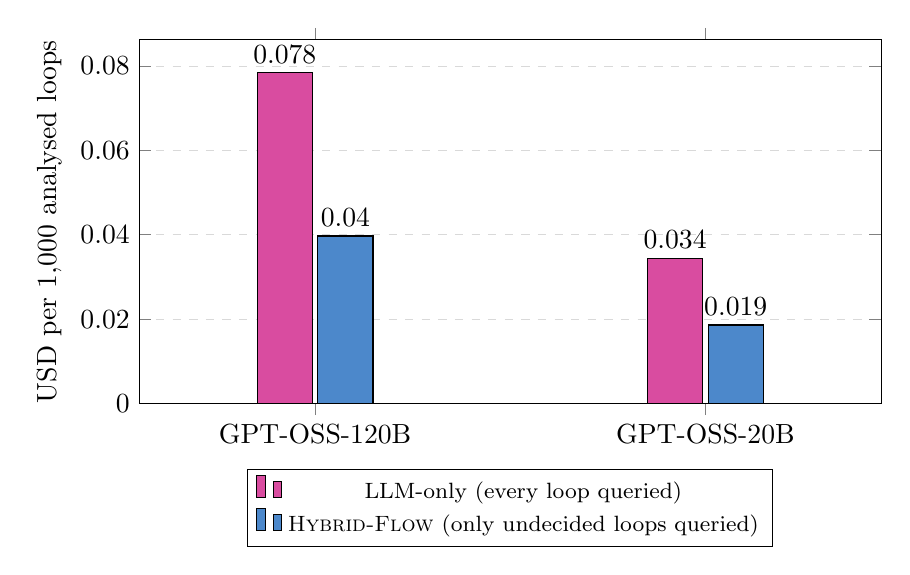
\begin{tikzpicture}
\begin{axis}[
    ybar, bar width=0.7cm, width=11cm, height=6.2cm, ymin=0, scaled y ticks=false, yticklabel style={/pgf/number format/fixed, /pgf/number format/precision=2},
    ylabel={USD per 1{,}000 analysed loops}, symbolic x coords={GPT-OSS-120B,GPT-OSS-20B}, xtick=data,
    nodes near coords={\pgfmathprintnumber[fixed,precision=3]\pgfplotspointmeta}, nodes near coords align={vertical},
    legend style={at={(0.5,-0.18)}, anchor=north, legend columns=1, font=\footnotesize}, enlarge x limits=0.45,
    ymajorgrids=true, grid style={dashed, gray!30}]
\addplot[fill=pipelineMagenta!70, draw=black] coordinates {(GPT-OSS-120B,0.0784) (GPT-OSS-20B,0.0344)};
\addplot[fill=pipelineBlue!70, draw=black] coordinates {(GPT-OSS-120B,0.0397) (GPT-OSS-20B,0.0186)};
\legend{LLM-only (every loop queried), \SystemName{} (only undecided loops queried)}
\end{axis}
\end{tikzpicture}
\caption{Measured token cost per 1{,}000 analysed loops at on-demand list prices (evaluation set).}
\label{fig:cost}
\end{figure}

% ---- end generated/fig_cost ----

\subsubsection{Prompt engineering and ablation}
\label{sec:rq-prompt}
Table~\ref{tab:ablation} compares the four prompt variants with Qwen3.8-27B on \nAblLoops{} loops, using real API calls, together with the P2 results of the GPT-OSS models on the same loops. \ablationText{}
% ---- begin generated/tables/ablation ----
% generated by hf/report.py from results/metrics.json - do not edit by hand
\begin{table}[htbp]
\caption{Prompt ablation (AI-only, no compiler facts).}
\label{tab:ablation}
\centering
\small
\resizebox{\linewidth}{!}{%
\begin{tabular}{lllrrrrrrr}
\toprule
Model & Prompt & Set & Loops & Parse fail & FP & Prec. & Rec. & F1 & Tok./loop \\
\midrule
qwen3.8-27b & P1 & ablation & 120 & 12.5 & 1 & 97.8 & 54.9 & 70.3 & 490 \\
qwen3.8-27b & P2 & ablation & 120 & 0.0 & 0 & 100.0 & 82.9 & 90.7 & 293 \\
qwen3.8-27b & P3 & ablation & 120 & 0.0 & 0 & 100.0 & 84.1 & 91.4 & 368 \\
qwen3.8-27b & P4 & ablation & 120 & 0.0 & 0 & 100.0 & 84.1 & 91.4 & 332 \\
gpt-oss-120b & P2 & ablation(eval subset) & 120 & -- & 1 & 98.7 & 90.2 & 94.3 & -- \\
gpt-oss-20b & P2 & ablation(eval subset) & 120 & -- & 4 & 94.6 & 85.4 & 89.7 & -- \\
\bottomrule
\end{tabular}
}
\end{table}

% ---- end generated/tables/ablation ----

\paragraph{Run-to-run consistency} \consistencyText{}

\subsection{RQ5: Performance impact}
\label{sec:rq-perf}
We built every GT-parallel kernel of HF-LoopBench with 64$\times$ larger default problem sizes at \Code{-O2} and measured serial and OpenMP run time with \perfThreads{} threads (minimum of three runs). Of the \nPerfValid{} kernels with correct output, \perfFracGtOne{} run faster in parallel; the geometric-mean speedup is \perfGeo{}$\times$ (median \perfMedian{}$\times$, maximum \perfMax{}$\times$; Figure~\ref{fig:perf}). Many kernels touch only a few megabytes and finish in milliseconds, so thread start-up and memory bandwidth limit the gains; the figures characterize the benchmark rather than a tuned application. A practical comparison of the tools is the fraction of the total achievable time saving $\sum_L \max(0, T_\mathrm{ser}(L)-T_\mathrm{par}(L))$ that each tool's accepted loops capture: on all loops, HF-Static captures \covFullStatic{}, GCC \covFullGcc{}, Polly \covFullPolly{} and the complete hybrid with GPT-OSS-20B \covFullHTwenty{}. On HF-LoopBench-X the geometric-mean speedup of the \xPerfN{} parallel kernels is \xPerfGeo{}$\times$.
% ---- begin generated/fig_perf ----
% generated by hf/paper_extra.py - do not edit by hand

\begin{figure}[htbp]
\centering
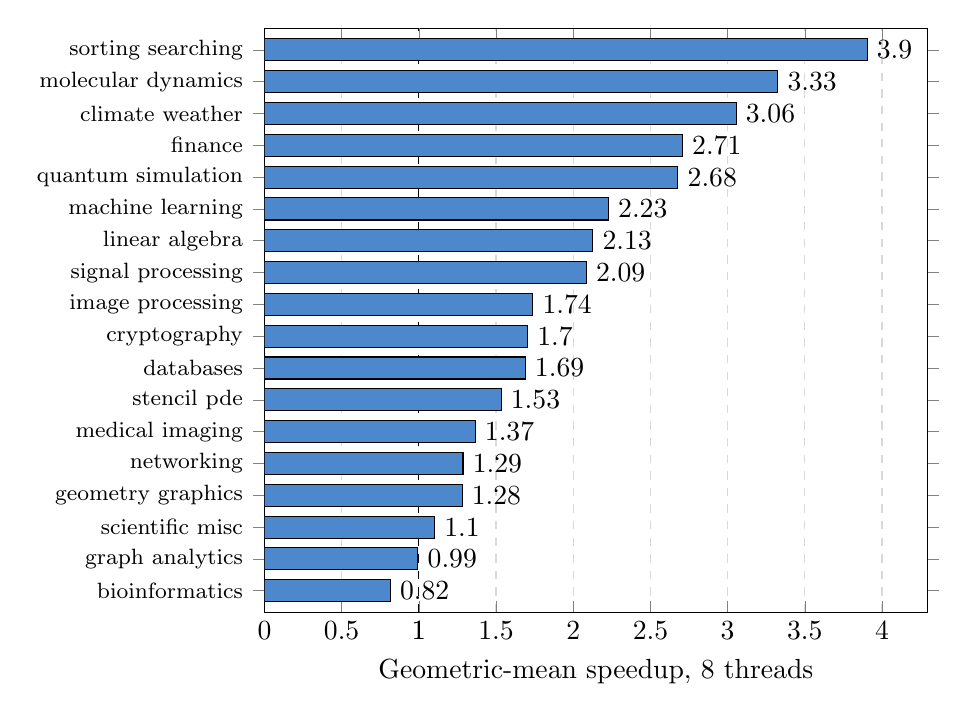
\begin{tikzpicture}
\begin{axis}[
    xbar, bar width=0.28cm, width=10cm, height=9cm, xmin=0,
    xlabel={Geometric-mean speedup, 8 threads}, symbolic y coords={bioinformatics,graph analytics,scientific misc,geometry graphics,networking,medical imaging,stencil pde,databases,cryptography,image processing,signal processing,linear algebra,machine learning,quantum simulation,finance,climate weather,molecular dynamics,sorting searching}, ytick=data, y tick label style={font=\footnotesize},
    nodes near coords={\pgfmathprintnumber[fixed,precision=2]\pgfplotspointmeta}, nodes near coords align={horizontal},
    xmajorgrids=true, grid style={dashed, gray!30}, enlarge y limits=0.04, extra x ticks={1}, extra x tick style={grid=major, grid style={black}}]
\addplot[fill=pipelineBlue!70, draw=black] coordinates {(3.903,sorting searching) (3.325,molecular dynamics) (3.055,climate weather) (2.707,finance) (2.678,quantum simulation) (2.228,machine learning) (2.127,linear algebra) (2.085,signal processing) (1.738,image processing) (1.704,cryptography) (1.689,databases) (1.533,stencil pde) (1.365,medical imaging) (1.286,networking) (1.280,geometry graphics) (1.102,scientific misc) (0.994,graph analytics) (0.815,bioinformatics)};
\end{axis}
\end{tikzpicture}
\caption{Speedup of the GT-parallel kernels of HF-LoopBench per domain (Apple M1 Pro, \Code{-O2}, minimum of three runs; kernels with wrong \Code{-O2} output excluded).}
\label{fig:perf}
\end{figure}

% ---- end generated/fig_perf ----

% ---- end sections/results ----
% ---- begin sections/cases ----
% =======================================================
% 7. CASE STUDIES
% =======================================================
\section{Case Studies}
\label{sec:cases}
The following cases are taken verbatim from the benchmarks; verdicts, confidences and explanations are quoted from the pass output and the request log.

\subsection{Case 1: 3-D stencil (affine but flattened access)}
\begin{lstlisting}[style=customc, caption={7-point Jacobi relaxation (\Code{st\_jacobi3d}, HF-LoopBench).}, label={lst:jacobi}]
for (int i = 1; i < n - 1; i++)
  for (int j = 1; j < n - 1; j++)
    for (int k = 1; k < n - 1; k++) {
      int c = (i * n + j) * n + k;
      un[c] = (u[c - n*n] + u[c + n*n] + u[c - n] + u[c + n]
               + u[c - 1] + u[c + 1]) / 6;
    }
\end{lstlisting}
\begin{itemize}
    \item \textit{LLVM analysis:} \textsc{Unknown} at all three levels, even for file-scope arrays: ``possible loop-carried output dependence (direction not resolved)''. The subscript \Code{c} is a linearized 3-D index, and DependenceAnalysis does not delinearize it, so it cannot show that different \Code{i} write different elements of \Code{un}. GCC rejects the nest as well; Polly, which reasons on the whole nest, accepts it.
    \item \textit{AI analysis:} GPT-OSS-20B and GPT-OSS-120B both answer ``parallel'' with \Code{collapse(3)} (confidence 0.98 and 0.96 with prompt P2), explaining that the stencil ``reads from a separate input array and writes to a distinct output array''.
    \item \textit{Hybrid verdict:} With GPT-OSS-20B ($\tau^*=\tauStarTwenty$) the directive is emitted; the oracle confirms it under all 12 configurations. With GPT-OSS-120B the compiler facts lower the model's confidence below its calibrated $\tau^*=\tauStarOneTwenty$ for the file-scope variant, and the loop is conservatively kept serial---a missed opportunity, not an error.
\end{itemize}

\subsection{Case 2: histogram (indirect access, legal only as an array reduction)}
\label{sec:case-hist}
\begin{lstlisting}[style=customc, caption={Grey-level histogram (\Code{im\_histogram}).}]
for (int i = 0; i < n; i++)
    hist[px[i]]++;
\end{lstlisting}
\begin{itemize}
    \item \textit{LLVM analysis:} \textsc{Unknown} (possible anti and output dependences through the indirect subscript); no tool proves anything here.
    \item \textit{AI analysis:} Both models answer ``serial'' with confidence 0.97--0.99 (``histogram bin increments create write-after-write races'').
    \item \textit{Hybrid verdict:} Serial, and therefore a missed opportunity: \Code{reduction(+:hist[:256])} makes the loop legal without touching its body, which the oracle verified. Our preliminary version described this pattern as rescued by the model through an \Code{atomic} directive; under the directive-only definition an atomic is a body modification, and in our data no model proposed the array-section reduction. Array reductions are the one parallel class that no method accepts (Table~\ref{tab:classes}).
\end{itemize}

\subsection{Case 3: failure mode of the LLM---the loop is fine, the call is not}
\begin{lstlisting}[style=customc, caption={An axpy kernel and the call that makes it serial (\Code{la\_axpy}, variant Q).}]
void la_axpy_dQ(double *y, const double *x, double alpha, int n) {
    for (int i = 0; i < n; i++)
        y[i] = alpha * x[i] + y[i];
}
...
la_axpy_dQ(lb + 1, lb, 1.5, 16384);   /* y overlaps x shifted by one */
\end{lstlisting}
\begin{itemize}
    \item \textit{LLVM analysis:} \textsc{Unknown} inside the callee (``dependence test inconclusive (may-alias)''); the call-site pass reports that \Code{y} and \Code{x} are derived from the same object.
    \item \textit{AI analysis:} Although the call is printed in the prompt, GPT-OSS-120B answers ``parallel'' with confidence 0.99 (``independent elementwise updates, no dependencies''), and so does GPT-OSS-20B, also with the compiler facts. This is the dominant hallucination in our data: \nAIFPQ{} of the \evAITwentyFP{} unsafe answers of GPT-OSS-20B are of this kind, and no threshold removes them because they are among the most confident answers.
    \item \textit{Hybrid verdict:} Vetoed by the call-site guard before the model is consulted. Without the guard, the hybrid would have emitted a race.
\end{itemize}

\subsection{Case 4: failure mode of the compiler---a soundness bug found by new loop shapes}
\begin{lstlisting}[style=customc, caption={Gather along a linked list stored as a successor array (\Code{x\_list\_walk}, HF-LoopBench-X).}]
int p = 0;
for (int k = 0; k < n; k++) {
    out[k] = val[p];
    p = nxt[p];
}
\end{lstlisting}
\begin{itemize}
    \item \textit{LLVM analysis (before the fix):} \textsc{Parallel} for the file-scope and \Code{restrict} variants. The latch value of the $\phi$-node of \Code{p} is a load from \Code{nxt}, which the loop never writes, and the pass treated such forwarded loads as benign.
    \item \textit{Execution oracle:} naive parallelization produces wrong output, so the label is confirmed serial.
    \item \textit{Resolution:} The load address depends on \Code{p} itself; the corrected rule (Algorithm~\ref{alg:static}, line~7) classifies the loop as a scalar recurrence, i.e.\ \textsc{Serial}. The case shows that a ``sound'' static stage is only as sound as its implementation, and that an execution-validated benchmark with deliberately unusual loop shapes is an effective way to test it.
\end{itemize}

% ---- end sections/cases ----
% ---- begin sections/discussion ----
% =======================================================
% 8. DISCUSSION AND THREATS TO VALIDITY
% =======================================================
\section{Discussion and Threats to Validity}
\label{sec:discussion}

\paragraph{What the model contributes, and what it must not decide} The data support a division of labour rather than a ranking. On loops whose independence is a matter of \emph{recognizing intent}---a stencil written with flattened indices, a gather through a lookup table, a temporary declared outside the loop, a DOALL loop over pointer parameters that are never overlapped---current open-weight models are far more complete than a sound compiler analysis. On loops whose legality depends on \emph{facts outside the text of the loop}---which arguments a caller passes, whether an index array is a permutation---they answer from the loop body alone and are confidently wrong. The static veto handles the second category when the fact is a proven dependence, and the call-site guard handles it when the fact is visible at a call in the same translation unit. Facts that are invisible to both (an index array that is a permutation only by construction, a pointer passed across translation units) remain the residual risk of any hybrid scheme, and are the reason we keep the threshold and the veto explicit and auditable.

\paragraph{Confidence is a weak gate} Self-reported confidence separated correct from incorrect answers only partially (Table~\ref{tab:aidist}), and for GPT-OSS-120B the compiler facts lowered the reported confidence without improving correctness. A threshold must therefore be calibrated on held-out data for each model and prompt; an evaluation that tunes it on the test set, as our preliminary version did, overstates both safety and recall.

\paragraph{Practical deployment} In a CI/CD setting HF-Static runs at compiler speed, so the cost of the pipeline is dominated by the model calls on \textsc{Unknown} loops; on realistic C++ these are about half of all loops (Table~\ref{tab:pipeline}). The measured cost is a fraction of a cent per loop, and exact-match caching of answers for unchanged code is safe, but similarity-based caching should not be used for legality decisions. Since the harness exposed both a miscompilation in the toolchain and a soundness bug in our own analysis, every directive proposed by any tool should be validated by differential execution before it is merged; for kernel-sized code this is inexpensive.

\paragraph{Limitations of HF-Static} The analysis is intra-procedural (apart from the call-site guard), works on optimized IR rather than on source, and inherits the precision of LLVM's DependenceAnalysis, which does not delinearize flattened subscripts. Delinearization, polyhedral dependence testing on static control parts and inter-procedural mod/ref information would move loops from \textsc{Unknown} to \textsc{Parallel} and reduce the work left to the model. The call-site guard vetoes legal calls with disjoint halves of one buffer; a range-based overlap test would remove these false vetoes.

\subsection{Threats to validity}
\label{sec:threats}

\paragraph{Construct validity} Our legality definition (one loop-level directive, unchanged body) is stricter than ``can be parallelized after restructuring''. Some loops labelled serial admit a parallel scan, a loop-nest transformation or run-time alias checks; a tool that performs such rewrites (Polly transforms six of these nests) is penalized by our metrics. Conversely, a parallel label is supported by 12 executions, not by a proof; the schedules were chosen to maximize interleavings, and every canonical serial loop of HF-LoopBench did produce a deviating result under naive parallelization, which indicates that the harness is sensitive to the dependences it is meant to expose. The arg-min loops of HF-LoopBench-X are serial by definition but their race did not manifest.

\paragraph{Internal validity} Ground-truth labels were written by the authors, and the benchmarks were designed together with the tools. To limit this bias, the HF-Static rules and prompts were fixed before the LLM experiments and not changed after observing model outputs, labels were validated by execution, the threshold was selected on a development split disjoint (by base kernel) from the reported test split, and HF-LoopBench-X was written after all of this was frozen. The only change after freezing is the soundness fix of Section~\ref{sec:rq-ext}, which can only turn verdicts into \textsc{Serial}; we report its effect on every corpus. LLM outputs are not fully deterministic even at temperature~0; we quantify run-to-run agreement and release the complete request/response log, from which every number is recomputed.

\paragraph{External validity} The benchmarks consist of small kernels with one target loop each and generated variants; real applications contain larger functions, macros, C++ abstractions and inter-procedural effects. The 200-file corpus shows that the pipeline scales to such code but has no ground truth. The LLM study is limited by free-tier quotas and to three open-weight models available on one provider at the time of the study; the Llama~3.3~70B model of our preliminary version is no longer served there. All timings come from one laptop-class processor.

% ---- end sections/discussion ----
% ---- begin sections/conclusion ----
% =======================================================
% 9. CONCLUSION
% =======================================================
\section{Conclusion}
\label{sec:conclusion}
This study re-evaluated LLM-assisted loop parallelization with execution-validated ground truth. A sound LLVM~21 analysis decided serial loops reliably but proved only \fsStaticRec{} of the parallel loops of HF-LoopBench. Open-weight LLMs used alone found most of the remaining parallelism yet issued unsafe directives for up to \evAITwentyFP{} of \nEvalLoops{} loops, mainly by ignoring how a function is called. Gating the model behind the compiler's three-valued verdict, a static veto and a call-site alias guard, and querying it only for the loops the compiler cannot decide, yielded F1 \evHCTwentyFone{} with no unsafe directive on the evaluation set, \fhTwentyFone{} with \fhTwentyFP{} unsafe directives on all \nBenchLoops{} loops, and F1 \xHTwentyFone{} on loop shapes written after the study was frozen, at a token cost \projSaveTwenty{} below that of LLM-only classification. The central design decisions---a veto the model cannot override, a threshold calibrated on held-out data, exact rather than similarity-based caching, and execution-based validation of every proposed directive---are what make the approach usable in a modernization pipeline.

\section*{Data and code availability}
\label{sec:artifact}
The implementation (LLVM plugin, Python driver), HF-LoopBench and HF-LoopBench-X with their generator and oracle, all raw results (oracle runs, static records, compiler-baseline output, the complete LLM request/response logs, timings) and the scripts that regenerate every table, figure and number of this article are available at \url{https://github.com/hoangtrietdev/llvm-analyze} (directory \Code{hybridflow/}). \Code{python3 run\_all.py analyze} recomputes all results from the logged data without contacting any API.

\section*{Acknowledgment}
\textit{Declaration of generative AI use:} The evaluated method uses the GPT-OSS-120B, GPT-OSS-20B and Qwen3.8-27B models via the Groq API. During the preparation of this work the authors used AI assistants (GitHub Copilot, Claude, Gemini) for code completion, debugging and editing of the manuscript. The authors reviewed and verified all code, data and text and take full responsibility for the content of the publication.

% ---- end sections/conclusion ----
% ---- begin sections/references ----
\bibliographystyle{elsarticle-num}
\begin{thebibliography}{99}
\bibitem{sutter2005} H. Sutter, The free lunch is over: a fundamental turn toward concurrency in software, Dr. Dobb's Journal 30 (3) (2005).
\bibitem{flynn2007} M. J. Flynn, Scaling, parallelism, and the impact of the processor-memory barrier, ACM Turing Lecture, SC 2007.
\bibitem{dongarra2023} J. Dongarra et al., A report on the Exascale Computing Project, International Journal of High Performance Computing Applications (2023).
\bibitem{banerjee1988} U. Banerjee, Dependence Analysis for Supercomputing, Kluwer, 1988.
\bibitem{pugh1992} W. Pugh, A practical algorithm for exact array dependence analysis, Communications of the ACM 35 (8) (1992) 102--114.
\bibitem{feautrier1991} P. Feautrier, Dataflow analysis of array and scalar references, International Journal of Parallel Programming 20 (1) (1991) 23--53.
\bibitem{bondhugula2008} U. Bondhugula, A. Hartono, J. Ramanujam, P. Sadayappan, A practical automatic polyhedral parallelizer and locality optimizer, in: PLDI, 2008, pp. 101--113.
\bibitem{grosser2012} T. Grosser, A. Gr\"o{\ss}linger, C. Lengauer, Polly -- performing polyhedral optimizations on a low-level intermediate representation, Parallel Processing Letters 22 (4) (2012) 1250010.
\bibitem{lattner2004} C. Lattner, V. Adve, LLVM: A compilation framework for lifelong program analysis \& transformation, in: CGO, 2004, pp. 75--86.
\bibitem{pop2005} S. Pop, A. Cohen, G.-A. Silber, Induction variable analysis with delayed abstractions, in: HiPEAC, LNCS 3793, 2005, pp. 218--232.
\bibitem{llvmda} LLVM Project, DependenceAnalysis and ScalarEvolution, LLVM 21 documentation, \url{https://llvm.org/docs/} (accessed 15 November 2026).
\bibitem{gccparloops} GCC Project, Auto-parallelization (\texttt{-ftree-parallelize-loops}), GCC documentation, \url{https://gcc.gnu.org/onlinedocs/} (accessed 15 November 2026).
\bibitem{li2016discopop} Z. Li, R. Atre, Z. Huda, A. Jannesari, F. Wolf, Unveiling parallelization opportunities in sequential programs, Journal of Systems and Software 117 (2016) 282--295.
\bibitem{harel2023pragformer} R. Harel, Y. Pinter, G. Oren, Learning to parallelize in a shared-memory environment with transformers, arXiv:2204.12835 (2022).
\bibitem{kadosh2023ompify} T. Kadosh, N. Schneider, N. Hasabnis, T. Mattson, Y. Pinter, G. Oren, Advising OpenMP parallelization via a graph-based approach with transformers, in: IWOMP, LNCS 14114, Springer, 2023, pp. 3--17.
\bibitem{kadosh2024ompar} T. Kadosh, N. Hasabnis, P. Soundararajan, V. A. Vo, M. Capota, N. Ahmed, Y. Pinter, G. Oren, OMPar: Automatic parallelization with AI-driven source-to-source compilation, arXiv:2409.14771 (2024).
\bibitem{chen2023graph2par} L. Chen, Q. I. Mahmud, H. Phan, N. K. Ahmed, A. Jannesari, Learning to parallelize with OpenMP by augmented heterogeneous AST representation, in: MLSys, 2023.
\bibitem{mahmud2025autoparllm} Q. I. Mahmud, A. TehraniJamsaz, H. Phan, L. Chen, M. Capot\u{a}, T. Willke, N. K. Ahmed, A. Jannesari, AutoParLLM: GNN-guided context generation for zero-shot code parallelization using LLMs, in: NAACL, 2025, pp. 11821--11841.
\bibitem{nichols2024pareval} D. Nichols, J. H. Davis, Z. Xie, A. Rajaram, A. Bhatele, Can large language models write parallel code?, in: HPDC, 2024.
\bibitem{taneja2025llmvectorizer} J. Taneja, A. Laird, C. Yan, M. Musuvathi, S. K. Lahiri, LLM-Vectorizer: LLM-based verified loop vectorizer, in: CGO, 2025.
\bibitem{pearce2022asleep} H. Pearce, B. Ahmad, B. Tan, B. Dolan-Gavitt, R. Karri, Asleep at the keyboard? Assessing the security of GitHub Copilot's code contributions, in: IEEE S\&P, 2022, pp. 754--768.
\bibitem{liao2017dataracebench} C. Liao, P.-H. Lin, J. Asplund, M. Schordan, I. Karlin, DataRaceBench: A benchmark suite for systematic evaluation of data race detection tools, in: SC, 2017.
\bibitem{pouchet2012} L.-N. Pouchet, PolyBench: The polyhedral benchmark suite, \url{https://sourceforge.net/projects/polybench/} (2012).
\bibitem{openmp52} OpenMP Architecture Review Board, OpenMP Application Programming Interface, Version 5.2, 2021.
\end{thebibliography}

% ---- end sections/references ----

\end{document}
